\documentclass{article} % For LaTeX2e
\usepackage{iclr2022_conference,times}

% Optional math commands from https://github.com/goodfeli/dlbook_notation.
%%%%% NEW MATH DEFINITIONS %%%%%

\usepackage{amsmath,amsfonts,bm}

% Mark sections of captions for referring to divisions of figures
\newcommand{\figleft}{{\em (Left)}}
\newcommand{\figcenter}{{\em (Center)}}
\newcommand{\figright}{{\em (Right)}}
\newcommand{\figtop}{{\em (Top)}}
\newcommand{\figbottom}{{\em (Bottom)}}
\newcommand{\captiona}{{\em (a)}}
\newcommand{\captionb}{{\em (b)}}
\newcommand{\captionc}{{\em (c)}}
\newcommand{\captiond}{{\em (d)}}

% Highlight a newly defined term
\newcommand{\newterm}[1]{{\bf #1}}


% Figure reference, lower-case.
\def\figref#1{figure~\ref{#1}}
% Figure reference, capital. For start of sentence
\def\Figref#1{Figure~\ref{#1}}
\def\twofigref#1#2{figures \ref{#1} and \ref{#2}}
\def\quadfigref#1#2#3#4{figures \ref{#1}, \ref{#2}, \ref{#3} and \ref{#4}}
% Section reference, lower-case.
\def\secref#1{section~\ref{#1}}
% Section reference, capital.
\def\Secref#1{Section~\ref{#1}}
% Reference to two sections.
\def\twosecrefs#1#2{sections \ref{#1} and \ref{#2}}
% Reference to three sections.
\def\secrefs#1#2#3{sections \ref{#1}, \ref{#2} and \ref{#3}}
% Reference to an equation, lower-case.
\def\eqref#1{equation~\ref{#1}}
% Reference to an equation, upper case
\def\Eqref#1{Equation~\ref{#1}}
% A raw reference to an equation---avoid using if possible
\def\plaineqref#1{\ref{#1}}
% Reference to a chapter, lower-case.
\def\chapref#1{chapter~\ref{#1}}
% Reference to an equation, upper case.
\def\Chapref#1{Chapter~\ref{#1}}
% Reference to a range of chapters
\def\rangechapref#1#2{chapters\ref{#1}--\ref{#2}}
% Reference to an algorithm, lower-case.
\def\algref#1{algorithm~\ref{#1}}
% Reference to an algorithm, upper case.
\def\Algref#1{Algorithm~\ref{#1}}
\def\twoalgref#1#2{algorithms \ref{#1} and \ref{#2}}
\def\Twoalgref#1#2{Algorithms \ref{#1} and \ref{#2}}
% Reference to a part, lower case
\def\partref#1{part~\ref{#1}}
% Reference to a part, upper case
\def\Partref#1{Part~\ref{#1}}
\def\twopartref#1#2{parts \ref{#1} and \ref{#2}}

\def\ceil#1{\lceil #1 \rceil}
\def\floor#1{\lfloor #1 \rfloor}
\def\1{\bm{1}}
\newcommand{\train}{\mathcal{D}}
\newcommand{\valid}{\mathcal{D_{\mathrm{valid}}}}
\newcommand{\test}{\mathcal{D_{\mathrm{test}}}}

\def\eps{{\epsilon}}


% Random variables
\def\reta{{\textnormal{$\eta$}}}
\def\ra{{\textnormal{a}}}
\def\rb{{\textnormal{b}}}
\def\rc{{\textnormal{c}}}
\def\rd{{\textnormal{d}}}
\def\re{{\textnormal{e}}}
\def\rf{{\textnormal{f}}}
\def\rg{{\textnormal{g}}}
\def\rh{{\textnormal{h}}}
\def\ri{{\textnormal{i}}}
\def\rj{{\textnormal{j}}}
\def\rk{{\textnormal{k}}}
\def\rl{{\textnormal{l}}}
% rm is already a command, just don't name any random variables m
\def\rn{{\textnormal{n}}}
\def\ro{{\textnormal{o}}}
\def\rp{{\textnormal{p}}}
\def\rq{{\textnormal{q}}}
\def\rr{{\textnormal{r}}}
\def\rs{{\textnormal{s}}}
\def\rt{{\textnormal{t}}}
\def\ru{{\textnormal{u}}}
\def\rv{{\textnormal{v}}}
\def\rw{{\textnormal{w}}}
\def\rx{{\textnormal{x}}}
\def\ry{{\textnormal{y}}}
\def\rz{{\textnormal{z}}}

% Random vectors
\def\rvepsilon{{\mathbf{\epsilon}}}
\def\rvtheta{{\mathbf{\theta}}}
\def\rva{{\mathbf{a}}}
\def\rvb{{\mathbf{b}}}
\def\rvc{{\mathbf{c}}}
\def\rvd{{\mathbf{d}}}
\def\rve{{\mathbf{e}}}
\def\rvf{{\mathbf{f}}}
\def\rvg{{\mathbf{g}}}
\def\rvh{{\mathbf{h}}}
\def\rvu{{\mathbf{i}}}
\def\rvj{{\mathbf{j}}}
\def\rvk{{\mathbf{k}}}
\def\rvl{{\mathbf{l}}}
\def\rvm{{\mathbf{m}}}
\def\rvn{{\mathbf{n}}}
\def\rvo{{\mathbf{o}}}
\def\rvp{{\mathbf{p}}}
\def\rvq{{\mathbf{q}}}
\def\rvr{{\mathbf{r}}}
\def\rvs{{\mathbf{s}}}
\def\rvt{{\mathbf{t}}}
\def\rvu{{\mathbf{u}}}
\def\rvv{{\mathbf{v}}}
\def\rvw{{\mathbf{w}}}
\def\rvx{{\mathbf{x}}}
\def\rvy{{\mathbf{y}}}
\def\rvz{{\mathbf{z}}}

% Elements of random vectors
\def\erva{{\textnormal{a}}}
\def\ervb{{\textnormal{b}}}
\def\ervc{{\textnormal{c}}}
\def\ervd{{\textnormal{d}}}
\def\erve{{\textnormal{e}}}
\def\ervf{{\textnormal{f}}}
\def\ervg{{\textnormal{g}}}
\def\ervh{{\textnormal{h}}}
\def\ervi{{\textnormal{i}}}
\def\ervj{{\textnormal{j}}}
\def\ervk{{\textnormal{k}}}
\def\ervl{{\textnormal{l}}}
\def\ervm{{\textnormal{m}}}
\def\ervn{{\textnormal{n}}}
\def\ervo{{\textnormal{o}}}
\def\ervp{{\textnormal{p}}}
\def\ervq{{\textnormal{q}}}
\def\ervr{{\textnormal{r}}}
\def\ervs{{\textnormal{s}}}
\def\ervt{{\textnormal{t}}}
\def\ervu{{\textnormal{u}}}
\def\ervv{{\textnormal{v}}}
\def\ervw{{\textnormal{w}}}
\def\ervx{{\textnormal{x}}}
\def\ervy{{\textnormal{y}}}
\def\ervz{{\textnormal{z}}}

% Random matrices
\def\rmA{{\mathbf{A}}}
\def\rmB{{\mathbf{B}}}
\def\rmC{{\mathbf{C}}}
\def\rmD{{\mathbf{D}}}
\def\rmE{{\mathbf{E}}}
\def\rmF{{\mathbf{F}}}
\def\rmG{{\mathbf{G}}}
\def\rmH{{\mathbf{H}}}
\def\rmI{{\mathbf{I}}}
\def\rmJ{{\mathbf{J}}}
\def\rmK{{\mathbf{K}}}
\def\rmL{{\mathbf{L}}}
\def\rmM{{\mathbf{M}}}
\def\rmN{{\mathbf{N}}}
\def\rmO{{\mathbf{O}}}
\def\rmP{{\mathbf{P}}}
\def\rmQ{{\mathbf{Q}}}
\def\rmR{{\mathbf{R}}}
\def\rmS{{\mathbf{S}}}
\def\rmT{{\mathbf{T}}}
\def\rmU{{\mathbf{U}}}
\def\rmV{{\mathbf{V}}}
\def\rmW{{\mathbf{W}}}
\def\rmX{{\mathbf{X}}}
\def\rmY{{\mathbf{Y}}}
\def\rmZ{{\mathbf{Z}}}

% Elements of random matrices
\def\ermA{{\textnormal{A}}}
\def\ermB{{\textnormal{B}}}
\def\ermC{{\textnormal{C}}}
\def\ermD{{\textnormal{D}}}
\def\ermE{{\textnormal{E}}}
\def\ermF{{\textnormal{F}}}
\def\ermG{{\textnormal{G}}}
\def\ermH{{\textnormal{H}}}
\def\ermI{{\textnormal{I}}}
\def\ermJ{{\textnormal{J}}}
\def\ermK{{\textnormal{K}}}
\def\ermL{{\textnormal{L}}}
\def\ermM{{\textnormal{M}}}
\def\ermN{{\textnormal{N}}}
\def\ermO{{\textnormal{O}}}
\def\ermP{{\textnormal{P}}}
\def\ermQ{{\textnormal{Q}}}
\def\ermR{{\textnormal{R}}}
\def\ermS{{\textnormal{S}}}
\def\ermT{{\textnormal{T}}}
\def\ermU{{\textnormal{U}}}
\def\ermV{{\textnormal{V}}}
\def\ermW{{\textnormal{W}}}
\def\ermX{{\textnormal{X}}}
\def\ermY{{\textnormal{Y}}}
\def\ermZ{{\textnormal{Z}}}

% Vectors
\def\vzero{{\bm{0}}}
\def\vone{{\bm{1}}}
\def\vmu{{\bm{\mu}}}
\def\vtheta{{\bm{\theta}}}
\def\va{{\bm{a}}}
\def\vb{{\bm{b}}}
\def\vc{{\bm{c}}}
\def\vd{{\bm{d}}}
\def\ve{{\bm{e}}}
\def\vf{{\bm{f}}}
\def\vg{{\bm{g}}}
\def\vh{{\bm{h}}}
\def\vi{{\bm{i}}}
\def\vj{{\bm{j}}}
\def\vk{{\bm{k}}}
\def\vl{{\bm{l}}}
\def\vm{{\bm{m}}}
\def\vn{{\bm{n}}}
\def\vo{{\bm{o}}}
\def\vp{{\bm{p}}}
\def\vq{{\bm{q}}}
\def\vr{{\bm{r}}}
\def\vs{{\bm{s}}}
\def\vt{{\bm{t}}}
\def\vu{{\bm{u}}}
\def\vv{{\bm{v}}}
\def\vw{{\bm{w}}}
\def\vx{{\bm{x}}}
\def\vy{{\bm{y}}}
\def\vz{{\bm{z}}}

% Elements of vectors
\def\evalpha{{\alpha}}
\def\evbeta{{\beta}}
\def\evepsilon{{\epsilon}}
\def\evlambda{{\lambda}}
\def\evomega{{\omega}}
\def\evmu{{\mu}}
\def\evpsi{{\psi}}
\def\evsigma{{\sigma}}
\def\evtheta{{\theta}}
\def\eva{{a}}
\def\evb{{b}}
\def\evc{{c}}
\def\evd{{d}}
\def\eve{{e}}
\def\evf{{f}}
\def\evg{{g}}
\def\evh{{h}}
\def\evi{{i}}
\def\evj{{j}}
\def\evk{{k}}
\def\evl{{l}}
\def\evm{{m}}
\def\evn{{n}}
\def\evo{{o}}
\def\evp{{p}}
\def\evq{{q}}
\def\evr{{r}}
\def\evs{{s}}
\def\evt{{t}}
\def\evu{{u}}
\def\evv{{v}}
\def\evw{{w}}
\def\evx{{x}}
\def\evy{{y}}
\def\evz{{z}}

% Matrix
\def\mA{{\bm{A}}}
\def\mB{{\bm{B}}}
\def\mC{{\bm{C}}}
\def\mD{{\bm{D}}}
\def\mE{{\bm{E}}}
\def\mF{{\bm{F}}}
\def\mG{{\bm{G}}}
\def\mH{{\bm{H}}}
\def\mI{{\bm{I}}}
\def\mJ{{\bm{J}}}
\def\mK{{\bm{K}}}
\def\mL{{\bm{L}}}
\def\mM{{\bm{M}}}
\def\mN{{\bm{N}}}
\def\mO{{\bm{O}}}
\def\mP{{\bm{P}}}
\def\mQ{{\bm{Q}}}
\def\mR{{\bm{R}}}
\def\mS{{\bm{S}}}
\def\mT{{\bm{T}}}
\def\mU{{\bm{U}}}
\def\mV{{\bm{V}}}
\def\mW{{\bm{W}}}
\def\mX{{\bm{X}}}
\def\mY{{\bm{Y}}}
\def\mZ{{\bm{Z}}}
\def\mBeta{{\bm{\beta}}}
\def\mPhi{{\bm{\Phi}}}
\def\mLambda{{\bm{\Lambda}}}
\def\mSigma{{\bm{\Sigma}}}

% Tensor
\DeclareMathAlphabet{\mathsfit}{\encodingdefault}{\sfdefault}{m}{sl}
\SetMathAlphabet{\mathsfit}{bold}{\encodingdefault}{\sfdefault}{bx}{n}
\newcommand{\tens}[1]{\bm{\mathsfit{#1}}}
\def\tA{{\tens{A}}}
\def\tB{{\tens{B}}}
\def\tC{{\tens{C}}}
\def\tD{{\tens{D}}}
\def\tE{{\tens{E}}}
\def\tF{{\tens{F}}}
\def\tG{{\tens{G}}}
\def\tH{{\tens{H}}}
\def\tI{{\tens{I}}}
\def\tJ{{\tens{J}}}
\def\tK{{\tens{K}}}
\def\tL{{\tens{L}}}
\def\tM{{\tens{M}}}
\def\tN{{\tens{N}}}
\def\tO{{\tens{O}}}
\def\tP{{\tens{P}}}
\def\tQ{{\tens{Q}}}
\def\tR{{\tens{R}}}
\def\tS{{\tens{S}}}
\def\tT{{\tens{T}}}
\def\tU{{\tens{U}}}
\def\tV{{\tens{V}}}
\def\tW{{\tens{W}}}
\def\tX{{\tens{X}}}
\def\tY{{\tens{Y}}}
\def\tZ{{\tens{Z}}}


% Graph
\def\gA{{\mathcal{A}}}
\def\gB{{\mathcal{B}}}
\def\gC{{\mathcal{C}}}
\def\gD{{\mathcal{D}}}
\def\gE{{\mathcal{E}}}
\def\gF{{\mathcal{F}}}
\def\gG{{\mathcal{G}}}
\def\gH{{\mathcal{H}}}
\def\gI{{\mathcal{I}}}
\def\gJ{{\mathcal{J}}}
\def\gK{{\mathcal{K}}}
\def\gL{{\mathcal{L}}}
\def\gM{{\mathcal{M}}}
\def\gN{{\mathcal{N}}}
\def\gO{{\mathcal{O}}}
\def\gP{{\mathcal{P}}}
\def\gQ{{\mathcal{Q}}}
\def\gR{{\mathcal{R}}}
\def\gS{{\mathcal{S}}}
\def\gT{{\mathcal{T}}}
\def\gU{{\mathcal{U}}}
\def\gV{{\mathcal{V}}}
\def\gW{{\mathcal{W}}}
\def\gX{{\mathcal{X}}}
\def\gY{{\mathcal{Y}}}
\def\gZ{{\mathcal{Z}}}

% Sets
\def\sA{{\mathbb{A}}}
\def\sB{{\mathbb{B}}}
\def\sC{{\mathbb{C}}}
\def\sD{{\mathbb{D}}}
% Don't use a set called E, because this would be the same as our symbol
% for expectation.
\def\sF{{\mathbb{F}}}
\def\sG{{\mathbb{G}}}
\def\sH{{\mathbb{H}}}
\def\sI{{\mathbb{I}}}
\def\sJ{{\mathbb{J}}}
\def\sK{{\mathbb{K}}}
\def\sL{{\mathbb{L}}}
\def\sM{{\mathbb{M}}}
\def\sN{{\mathbb{N}}}
\def\sO{{\mathbb{O}}}
\def\sP{{\mathbb{P}}}
\def\sQ{{\mathbb{Q}}}
\def\sR{{\mathbb{R}}}
\def\sS{{\mathbb{S}}}
\def\sT{{\mathbb{T}}}
\def\sU{{\mathbb{U}}}
\def\sV{{\mathbb{V}}}
\def\sW{{\mathbb{W}}}
\def\sX{{\mathbb{X}}}
\def\sY{{\mathbb{Y}}}
\def\sZ{{\mathbb{Z}}}

% Entries of a matrix
\def\emLambda{{\Lambda}}
\def\emA{{A}}
\def\emB{{B}}
\def\emC{{C}}
\def\emD{{D}}
\def\emE{{E}}
\def\emF{{F}}
\def\emG{{G}}
\def\emH{{H}}
\def\emI{{I}}
\def\emJ{{J}}
\def\emK{{K}}
\def\emL{{L}}
\def\emM{{M}}
\def\emN{{N}}
\def\emO{{O}}
\def\emP{{P}}
\def\emQ{{Q}}
\def\emR{{R}}
\def\emS{{S}}
\def\emT{{T}}
\def\emU{{U}}
\def\emV{{V}}
\def\emW{{W}}
\def\emX{{X}}
\def\emY{{Y}}
\def\emZ{{Z}}
\def\emSigma{{\Sigma}}

% entries of a tensor
% Same font as tensor, without \bm wrapper
\newcommand{\etens}[1]{\mathsfit{#1}}
\def\etLambda{{\etens{\Lambda}}}
\def\etA{{\etens{A}}}
\def\etB{{\etens{B}}}
\def\etC{{\etens{C}}}
\def\etD{{\etens{D}}}
\def\etE{{\etens{E}}}
\def\etF{{\etens{F}}}
\def\etG{{\etens{G}}}
\def\etH{{\etens{H}}}
\def\etI{{\etens{I}}}
\def\etJ{{\etens{J}}}
\def\etK{{\etens{K}}}
\def\etL{{\etens{L}}}
\def\etM{{\etens{M}}}
\def\etN{{\etens{N}}}
\def\etO{{\etens{O}}}
\def\etP{{\etens{P}}}
\def\etQ{{\etens{Q}}}
\def\etR{{\etens{R}}}
\def\etS{{\etens{S}}}
\def\etT{{\etens{T}}}
\def\etU{{\etens{U}}}
\def\etV{{\etens{V}}}
\def\etW{{\etens{W}}}
\def\etX{{\etens{X}}}
\def\etY{{\etens{Y}}}
\def\etZ{{\etens{Z}}}

% The true underlying data generating distribution
\newcommand{\pdata}{p_{\rm{data}}}
% The empirical distribution defined by the training set
\newcommand{\ptrain}{\hat{p}_{\rm{data}}}
\newcommand{\Ptrain}{\hat{P}_{\rm{data}}}
% The model distribution
\newcommand{\pmodel}{p_{\rm{model}}}
\newcommand{\Pmodel}{P_{\rm{model}}}
\newcommand{\ptildemodel}{\tilde{p}_{\rm{model}}}
% Stochastic autoencoder distributions
\newcommand{\pencode}{p_{\rm{encoder}}}
\newcommand{\pdecode}{p_{\rm{decoder}}}
\newcommand{\precons}{p_{\rm{reconstruct}}}

\newcommand{\laplace}{\mathrm{Laplace}} % Laplace distribution

\newcommand{\E}{\mathbb{E}}
\newcommand{\Ls}{\mathcal{L}}
\newcommand{\R}{\mathbb{R}}
\newcommand{\emp}{\tilde{p}}
\newcommand{\lr}{\alpha}
\newcommand{\reg}{\lambda}
\newcommand{\rect}{\mathrm{rectifier}}
\newcommand{\softmax}{\mathrm{softmax}}
\newcommand{\sigmoid}{\sigma}
\newcommand{\softplus}{\zeta}
\newcommand{\KL}{D_{\mathrm{KL}}}
\newcommand{\Var}{\mathrm{Var}}
\newcommand{\standarderror}{\mathrm{SE}}
\newcommand{\Cov}{\mathrm{Cov}}
% Wolfram Mathworld says $L^2$ is for function spaces and $\ell^2$ is for vectors
% But then they seem to use $L^2$ for vectors throughout the site, and so does
% wikipedia.
\newcommand{\normlzero}{L^0}
\newcommand{\normlone}{L^1}
\newcommand{\normltwo}{L^2}
\newcommand{\normlp}{L^p}
\newcommand{\normmax}{L^\infty}

\newcommand{\parents}{Pa} % See usage in notation.tex. Chosen to match Daphne's book.

\DeclareMathOperator*{\argmax}{arg\,max}
\DeclareMathOperator*{\argmin}{arg\,min}

\DeclareMathOperator{\sign}{sign}
\DeclareMathOperator{\Tr}{Tr}
\let\ab\allowbreak

\newcommand{\real}[1]{\mathbb{R}^{#1}}

\newcommand{\imageDataset}{\mathcal{X}}
\newcommand{\image}{\mathbf{x}}
\newcommand{\pixel}[1]{x_{#1}}

\newcommand{\latentDataset}{\mathcal{L}}
\newcommand{\latent}{\mathbf{z}}

\newcommand{\vqganEncoder}{E}
\newcommand{\vqganDecoder}{G}
\newcommand{\vqganCodebook}{\mathcal{C}}
\newcommand{\vqganDownsample}{f}
\newcommand{\codebookVector}{\mathbf{e}}

\newcommand{\hourglassRate}{k}


\usepackage[pagebackref,breaklinks,colorlinks]{hyperref}
\usepackage{url}
\usepackage{svg}
\usepackage{pgfplots}

\pgfplotsset{width=10cm,compat=1.9}
%\usepgfplotslibrary{external}
%\tikzexternalize

% uncomment below for smaller margins
\usepackage[margin=1in]{geometry}

\usepackage{graphicx}
\usepackage{amsmath}
\usepackage{amssymb}
\usepackage{booktabs}
\usepackage{overpic}
\usepackage{caption}
\usepackage{subcaption}

% It is strongly recommended to use hyperref, especially for the review version.
% hyperref with option pagebackref eases the reviewers' job.
% Please disable hyperref *only* if you encounter grave issues, e.g. with the
% file validation for the camera-ready version.
%
% If you comment hyperref and then uncomment it, you should delete
% ReviewTempalte.aux before re-running LaTeX.
% (Or just hit 'q' on the first LaTeX run, let it finish, and you
%  should be clear).
\usepackage[pagebackref,breaklinks,colorlinks]{hyperref}
\usepackage[acronym]{glossaries}
\glsdisablehyper

\newacronym{sundae}{SUNDAE}{step-unrolled denoising autoencoders}
\newacronym{ar}{AR}{autoregressive}
\newacronym{nar}{NAR}{non-autoregressive}

\newacronym{gan}{GAN}{generative adversarial network}
\newacronym{vae}{VAE}{variational auto-encoder}
\newacronym{vq}{VQ}{vector-quantization}
\newacronym{sbm}{SBM}{score-based model}
\newacronym{ebm}{EBM}{energy-based model}

\newacronym{vqgan}{VQ-GAN}{vector-quantized \acrshort{gan}}
\newacronym{vqvae}{VQ-VAE}{vector-quantized \acrshort{vae}}


% Support for easy cross-referencing
\usepackage[capitalize]{cleveref}
\crefname{section}{Sec.}{Secs.}
\Crefname{section}{Section}{Sections}
\Crefname{table}{Table}{Tables}
\crefname{table}{Tab.}{Tabs.}

\title{Megapixel Image Generation with Step-unrolled Denoising Autoencoders}

% Authors must not appear in the submitted version. They should be hidden
% as long as the \iclrfinalcopy macro remains commented out below.
% Non-anonymous submissions will be rejected without review.

\author{Alex F. McKinney \& Chris G. Willcocks \\
Department of Computer Science\\
Durham University\\
Durham, UK \\
\texttt{\{alexander.f.mckinney,christopher.g.willcocks\}@durham.ac.uk} \\
}

% The \author macro works with any number of authors. There are two commands
% used to separate the names and addresses of multiple authors: \And and \AND.
%
% Using \And between authors leaves it to \LaTeX{} to determine where to break
% the lines. Using \AND forces a linebreak at that point. So, if \LaTeX{}
% puts 3 of 4 authors names on the first line, and the last on the second
% line, try using \AND instead of \And before the third author name.

\newcommand{\fix}{\marginpar{FIX}}
\newcommand{\new}{\marginpar{NEW}}

\iclrfinalcopy % Uncomment for camera-ready version, but NOT for submission.
\begin{document}

\maketitle

\begin{abstract}
    % Context + Problem (1-2 sentences), Solution (1 salient idea), Key
% findings/surprise/discovery (1 sentence), State-of-the-art-results 

% TODO: add some scores

Recent research has pushed sample resolutions higher whilst reducing
computational requirements and sampling speeds. One approach is to utilize
powerful vector-quantization (VQ) models to reduce computational requirements
whilst still producing high quality samples. In this work, we push this further
through the use of non-autoregressive (NAR) denoising autoencoders (SUNDAE) and
modifications to hierarchical transformers that have found recent success in
language modelling. This approach to allows for very fast sampling and training
(4-6 days) of VQ latents from pre-trained VQ-GAN models. Furthermore, we found
the NAR nature of the model made it suitable for complex
inpainting with arbitrary masks. Finally, we trained a new VQ-GAN model on a
dataset of faces at resolutions exceeding one million pixels, ultimately
allowing allowing for megapixel image generation in only two seconds.

%Advancements in deep generative modelling has pushed sample resolution higher
%whilst reducing computational requirements and sampling speeds. One approach
%works in two stages: training a powerful vector-quantization image model and
%then training a second discrete prior to predict discrete tokens corresponding
%to image patches. Early work produced high fidelity and diverse samples, but
%were prohibitively slow to sample from as they were autoregressive in nature.
%Later work exploited discrete diffusion models in order to allow for parallel
%token prediction, dramatically speeding up the sampling process. In this work,
%we push the sampling speed and computational requirements further by replacing
%discrete diffusion models with denoising autoencoders, as well as modifications
%to the Transformer backbone including axial embeddings, an hourglass structure,
%and resampling layers more suited to image tasks. Furthermore, the
%non-autoregressive nature of the model allows for arbitrary inpainting patterns.
%Finally, we train new vector-quantization models to allow for the sampling of
%upwards of a megapixel images in seconds, and without relying on sliding window
%mechanisms.


% Reference FYI from our recent submission that's similar to you (it's not the best abstract, a bit too wordy, but not too bad):
% Whilst diffusion probabilistic models can generate high quality image content, key limitations remain in terms of both generating high-resolution imagery and their associated high computational requirements. Recent Vector-Quantized image models have overcome this limitation of image resolution but are prohibitively slow and unidirectional as they generate tokens via element-wise autoregressive sampling from the prior. By contrast, in this paper we propose a novel discrete diffusion probabilistic model prior which enables parallel prediction of Vector-Quantized tokens by using an unconstrained Transformer architecture as the backbone. During training, tokens are randomly masked in an order-agnostic manner and the Transformer learns to predict the original tokens. This parallelism of Vector-Quantized token prediction in turn facilitates unconditional generation of globally consistent high-resolution and diverse imagery at a fraction of the computational expense. In this manner, we can generate image resolutions exceeding that of the original training set samples whilst additionally provisioning per-image likelihood estimates (in a departure from generative adversarial approaches). Our approach achieves state-of-the-art results in terms of Density (LSUN Bedroom: 1.51; LSUN Churches: 1.12; FFHQ: 1.20) and Coverage (LSUN Bedroom: 0.83; LSUN Churches: 0.73; FFHQ: 0.80), and performs competitively on FID (LSUN Bedroom: 3.64; LSUN Churches: 4.07; FFHQ: 6.11) whilst offering advantages in terms of both computation and reduced training set requirements.

\end{abstract}

% TODO; how do these timings compare with other SOTA AR and NAR models (aside
% from GANs)?
\begin{figure}[ht]
    \centering
    \makebox[\textwidth]{
        \includegraphics[width=1.0\textwidth]{figures/sample1024.png}
    }
    \caption{
        High-resolution samples produced using our non-autoregressive approach.
        Each $1024 \times 1024$ sample was generated in $\approx 2$ seconds on a
        GTX 1080Ti -- including both discrete latent sampling and subsequent
        decoding. The SUNDAE sampler was trained in 4 days on a single V100
        32GB.
    }
\end{figure}

\section{Introduction}\label{sec:intro}
An ideal deep generative model would satisfy three key requirements:
high-quality samples, sample diversity via mode coverage, and computational
inexpensive sampling. Arguably, there are other desirable properties such as a
meaningful latent space and exact likelihood calculation, however no current
generative model can satisfy all three requirements -- let alone additional
attractive properties -- thus forming the so-called generative modelling
trilemma~\cite{xiao2021trilemma}.

Models such as \glspl{gan}~\cite{goodfellow2014gan}
excel at high-quality and fast sampling, but often fail to model the entire data
distribution due to not directly optimising for likelihood -- using an
adversarial loss as a proxy. \Glspl{vae}~\cite{kingma2013vae} offer
excellent mode coverage and fast sampling speeds, but the resulting samples are
often blurry even at small resolutions, and have little hope of scaling to
greater resolutions like \glspl{gan}.

\Gls{ar} models such as PixelSnail~\cite{chen2017snail}, Image
Transformer~\cite{parmar2018image}, and DALL-E~\cite{parmar2018image} have
demonstrated respectable sample quality and mode coverage, even including
zero-shot image generation~\cite{ramesh2021dalle}. However, they are
computationally expensive to sample from, requiring many network iterations,
making them infeasible for interactive applications. \Glspl{ddpm}~\cite{ho2020ddpm}
and \glspl{sbm}~\cite{song2019sbm,song2020sde,song2021mlt} produce
samples that rival or even exceed the quality of \glspl{gan}~\cite{dhariwal2021ddpm}
whilst still providing good mode coverage, but are still plagued by potentially
requiring thousands of network evaluations.

Vector-quantized image
modelling~\cite{oord2017vqvae,razavi2019generating,esser2021taming} alleviates
sampling speed issues in \gls{ar} methods by reducing the spatial dimension at
which \gls{ar} sampling occurs. This results in excellent quality samples whilst
improving sampling speeds, but often requires a two-stage approach and still
does not match the speed of \glspl{gan}. Recent work has applied \gls{vq}
methods to diffusion models~\cite{bondtaylor2021unleashing} allowing for fast
parallel decoding. Other work does not use vector-quantized spaces, but latent
spaces nonetheless, to accelerate
sampling~\cite{xiao2021trilemma,vahdat2021sbmlatent}.

From this brief overview of generative modelling literature, it is clear that
indeed no single model satisfies all three conditions. This therefore motivates
research into explicitly addressing this trilemma. In this work, we move towards
such a solution, beginning from existing work applying generative models to
discrete latents. This provides an excellent starting point in terms of sample
quality and a respectable amount of mode coverage, but an unacceptably slow
sampling speed despite the reduced spatial dimension of the discrete latent
space. We directly address this issue by instead sampling discrete latents using
modern \gls{nar} generative models in an effort to close the gap, sampling speed
wise, with constant iteration complexity models such as \glspl{gan}.
Specifically, we use discrete \gls{sundae}~\cite{savinov2022stepunrolled} to
gradually denoise samples from a uniform prior into one that matches the prior
over the discrete latent space defined by a pre-trained \gls{vqgan} model. This
forms our first research question, whether \gls{sundae} models is suitable
paradigm for sampling discrete latent codes. As a result of our studies, we find
that indeed they are highly suited for this task.

These discrete \gls{sundae} models have only previously be applied to
language modelling tasks~\cite{savinov2022stepunrolled}. In their work, they
used transformer~\cite{vaswani2017attention} architectures to form their
autoencoder. In parallel, a noticeably more efficient variant of transformers --
the Hourglass Transformer~\cite{nawrot2021hierarchical} -- was released, which
has a hierarchical architecture aimed at language and image modelling tasks,
though potentially flawed on the latter. This raises a second research question,
whether the approach introduced in~\citet{savinov2022stepunrolled} is also
suited for latent modelling, and whether the hierarchical approach introduced
in~\citet{nawrot2021hierarchical} can be further improved upon. As a result of
our studies, we find that although they are suited for latent modelling, there
are many modifications we can make to improve their performance further.

Given a fast sampling and an efficient transformer architecture, we are
potentially left with a highly scaleable (with respect to spatial resolution)
model. This raises a third and final research question, whether our new approach
allows for the generation of extremely high resolution images in a time frame
that would permit fully-, or near-interactive use. Again, as a result of our
studies, we find that this is indeed the case, proven by the synthesis of $1024
\times 1024$ images in as few as 2 seconds on a consumer-grade GPU. To our
knowledge, this is the fastest sampling model at this resolution, with the
exception of pure \gls{gan}-based approaches. This required the training of our
own \gls{vqgan} model, which was, also to our knowledge, the largest \gls{vqgan} model
trained in terms of input size.

%In this work, we aim to move towards satisfying all three key requirements for
%an ideal generative model. Like previous work, we use a vector-quantized image
%model to reduce the spatial dimension of the signal we wish to sample. We then
%apply new language models to instead model the distribution of discrete latents,
%ultimately obtaining a powerful prior over the discrete latents. With this and a
%discrete latent decoder, we obtain the final generative model, allowing sampling
%of images in a very low number of steps. We go further, and train our own
%VQ-GAN~\cite{esser2021taming} at resolutions higher than ever trained before to
%our knowledge, ultimately allowing for the sampling of $1024 \times 1024$ RGB
%images in only two seconds on a consumer-grade GPU.

Our project objectives were as follows:
\begin{itemize}
    \item Apply \gls{sundae} to the task of \acrshort{vq} latent generation and
        ultimately image generation, and perform analysis into their advantages
        of being used for this task over existing approaches, including both
        \gls{ar} and \gls{nar} solutions.

    \item Analyse the methods used in \citet{savinov2022stepunrolled} and
        \citet{nawrot2021hierarchical} and design modifications that make these
        approaches more suitable for \acrshort{vq} latent modelling.

    \item Attempt to scale our model to extremely high resolution images and
        analyse successes and failures when operating at such resolutions. 

\end{itemize}


\section{Related Work}\label{sec:related}
% TODO: still needs narrative flow between sections

This work builds upon much prior research into powerful deep generative models,
self-supervised methods, and efficient transformer architectures. We cover
relevant prior work into deep generative models in
\S\ref{subsec:agm}-\ref{subsec:vqmodelling}, a specific \acrshort{nar}
generative model \gls{sundae} \S\ref{subsec:sundae}, and a recent development
into a efficient transformer architecture in \S\ref{subsec:hourglass}. For a
full review on generative modelling we direct the reader to
\citet{bondtaylor2021review}, and for further details on \gls{sundae} and
hourglass transformers to \citet{savinov2022stepunrolled} and
\citet{nawrot2021hierarchical} respectively.

\begin{figure}[ht!]
    \centering
    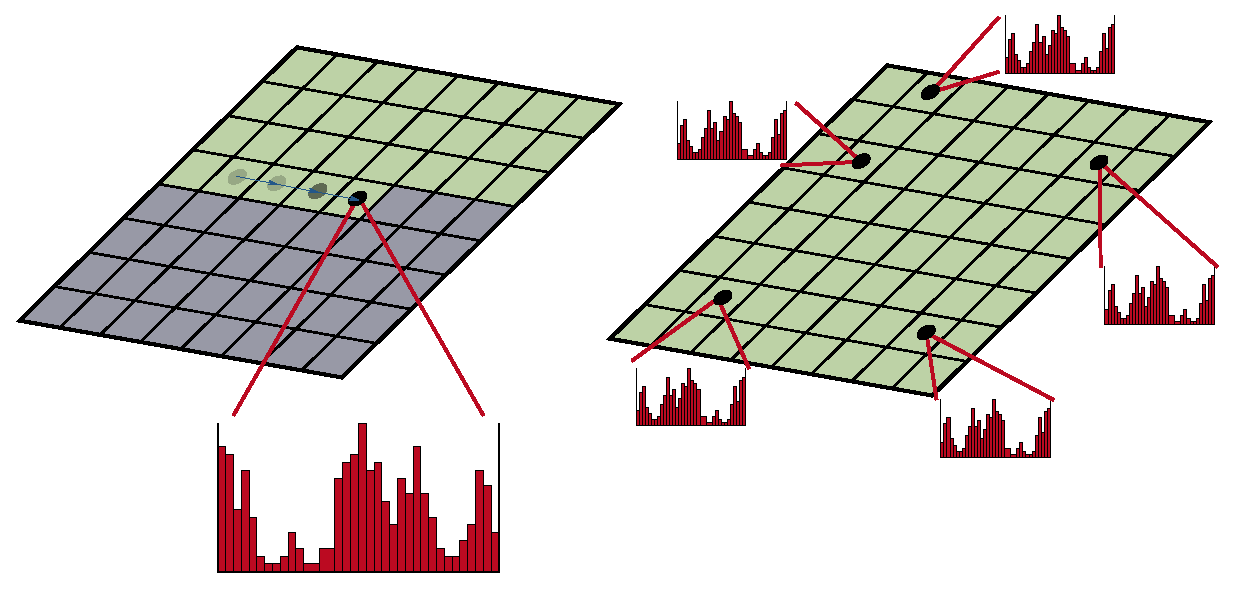
\includegraphics[width=\textwidth]{figures/AR-NAR.pdf}
    \caption{
        \textbf{Left:} Visualization of \acrfull{ar} sampling. \gls{ar} sampling
        proceeds one item at a time, resulting in the number of sampling steps
        being equal to the dimensionality of the input. For each prediction, a
        probability distribution over possible tokens is predicted and then
        sampled from. Each prediction can only make use of past context --
        indicated as a green position -- so not to violate the autoregressive
        property.
        \textbf{Right:} Visualization of \acrfull{nar} sampling. \gls{nar}
        sampling can sample an arbitrary number of items in parallel, including
        ones previously sampled, allowing for self-correction. It can freely use
        all context available to it, allowing for flexible inpainting and
        potentially better predictions.
    }
\end{figure}

\subsection{Autoregressive Generative Models}
\label{subsec:agm}

One major deep generative model family are \acrfull{ar} models, characterised by
a training and inference process based on the probabilistic chain rule. During
training, they learn to maximise the likelihood of the data they are
trained on, which leads to excellent mode coverage. Prior work using these
methods resulted in impressive results in terms of both sample quality and
diversity, but are ultimately impractical in real world applications due to
their slow sampling speed.

The slow sampling speed is due to their sequential nature, defined by the chain
rule of probability. Given an input $\image = \{ \pixel{1}, \pixel{2}, \dots,
\pixel{n} \}$, an \gls{ar} model $p_\theta(\cdot)$ generates new
samples sequentially:
\begin{equation}\label{eq:ar}
    p_\theta(\image) = p_\theta(\pixel{1}, \dots, \pixel{n}) =
    \prod\limits^{n}_{i=1} p_\theta(\pixel{i} \vert \pixel{1}, \dots, \pixel{i-1})
\end{equation}
meaning that the number of sampling steps is equal to the size of the
decomposition of $\image$, making this slow for large inputs.

For certain tasks, the ordering of the decomposition of $\image$ is obvious, for
example on text or speech. For images this is less obvious, however typically a
raster scan ordering is used~\cite{parmar2018image}. Certain \gls{ar} models are
order-agnostic~\cite{hoogeboom2021autoregressive}, allow for arbitrary ordering
to be used during training and inference.

One class of \gls{ar} models are \glspl{rnn} which are an early example of using
neural networks to model sequential data, such as text, audio, time-series data,
or even handwriting strokes. Though they can be used as classification or
regression models, they are also suited for use as generative models by
modelling the relationship in Equation~\ref{eq:ar}. They suffer from a number of
issues, most infamously vanishing gradients~\cite{pascanu2012rnn} and inability
to model long-range relationships between items in the input.
\Glspl{lstm}~\cite{hoch1997lstm} improved upon \glspl{rnn} further by
introducing dedicated memory units, allowing for the modelling of longer range
relationships. \Glspl{gru}~\cite{cho2014gru} simplified \gls{lstm} architecture
whilst retaining good performance. With the advent of transformer
architectures~\cite{vaswani2017attention}, modelling even longer relationships
became possible, even at a full-document level. It also introduced the
capability to train on all sequence elements in parallel through the use of
causal masking, therefore not violating the autoregressive property. Inference
must still be done in a serial manner, however.

Applying \gls{ar} models to images followed a similar trend.
PixelRNN~\cite{oord2016pixelrnn} used two-dimensional recurrent layers and
residual connections to model the distribution of raw pixel values. The same
paper also introduced PixelCNN, which was claimed to have worse performance but
were faster to train. These were extended to allow for conditional generation
in~\cite{oord2016pixelcnn}. Later work augmented PixelCNN with self-attention
mechanism, forming PixelSnail~\cite{chen2017snail}, which can model
longer relationships than a convolutional or recurrent architecture. Image
Transformer~\cite{parmar2018image} later applied transformer architectures to
the same task through an effective but conceptually simple approach.

\subsection{Non-autoregressive Generative Models}
\label{subsec:nagm}

\Acrfull{nar} generative models include \glspl{gan}, \glspl{sbm} and
\glspl{ddpm}, flow-based models, \glspl{ebm}, and implicit models. Though the
number of sampling steps is now independent of the data dimensionality (as we no
longer use the chain rule of probability to sample) the actual number of steps
required varies greatly: from single-step generation in \glspl{gan} to
potentially many thousands in early diffusion models.

Perhaps the most infamous class of \gls{nar} generative model -- or perhaps
generative model altogether -- are \acrfullpl{gan}~\cite{goodfellow2014gan}.
\Glspl{gan} consist of two models: a generator that creates images from a latent
variable, and a discriminator that attempts to distinguish images from the
dataset from images generated by the generator network~\cite{goodfellow2014gan}.
They are known for high-fidelity samples, fast sampling, unstable training, and
tendency to collapse onto a subset of modes of the underlying distribution due
to not optimising directly for likelihood. This is reflected in its relatively
low-diversity samples. Nonetheless, the quality of the samples has made them a
popular choice in a variety of applications, including unconditional and
conditional generation~\cite{tero2018stylegan,andrew2018biggan} image, audio
synthesis~\cite{liu2020audiogan}, and style transfer~\cite{zhu2017cyclegan}.
They can even be applied to discrete data~\cite{autume2019scratchgan}, but are
less effective on such domains due to the non-differentiability of discrete
samples.

Another class of generative model are \acrfullpl{vae}~\cite{kingma2013vae} which
permit sampling in a single forward pass like \glspl{gan}, but are trained to
maximise likelihood. Specifically, \glspl{vae} map inputs to latent variables
that follow some easy to sample from, but sufficiently complex, prior
distribution. A common choice is a multivariate Gaussian with diagonal
covariance~\cite{kingma2013vae}. A decoder network maps latent codes back
to the data distribution. Although this approach is successful on small
datasets, on more complex datasets the samples and reconstructions tend to
become blurry, suggesting a simple prior is unable to perfectly fit the
distribution. Later work extended \glspl{vae} to be hierarchical, having
multiple Gaussian priors~\cite{arash2020nvae,child2020vqvae} which were found to
outperform purely autoregressive models.

% TODO: add references for normalizing flows (eg. Glow)
Normalizing flows are another class of generative model that allows for exact
likelihood calculation~\cite{dinh2014nice,dinh2016density,kingma2018glow}. They
consist of many invertible layers that gradually transform samples from a known
prior distribution into samples from the data distribution. Each transformation
must satisfy two properties: being invertible and having an easy to compute
Jacobian for the purposes of scaling~\cite{dinh2014nice,dinh2016density}. This
makes the architectural choices restrictive, making them less parameter
efficient. They also typically must operate at the same dimensionality for each
layer, making the training of deep networks difficult.

Two paradigms of high interest in recent work are
\acrfullpl{ddpm}~\cite{ho2020ddpm,dhariwal2021ddpm} and
\acrfullpl{sbm}~\cite{song2019sbm,song2020sde,song2021mlt,vahdat2021sbmlatent}.
Both are variants of \glspl{ebm}, with the former learning to estimate the noise
at various levels (which can be used to iteratively move from noise to data),
and the latter trained to remove noise, given corrupted samples from a gradually
corrupting forward process. Again, this is then used to move from pure noise
back to data. Both are slow to sample from, but produce high quality samples
that rival those of \glspl{gan}~\cite{dhariwal2021ddpm} whilst not suffering
from mode collapse. The slow sampling speed can be remedied using a variety of
techniques, such as operating on a smaller latent
space~\cite{vahdat2021sbmlatent}, devising more efficient SDE
solvers~\cite{martineau2021fast}, or by diffusing ``velocities'', thus
simplifying the denoising task~\cite{dockhorn2021langevin}. Unlike \glspl{gan},
both models can operate on discrete data, such as by first projecting
discrete data into a continuous latent space~\cite{vahdat2021sbmlatent} or with
a dedicated discrete diffusion framework~\cite{austin2021structured}, the latter
of which bridges the gap between diffusion, autoregressive, and mask-based
representation models such as BERT~\cite{devlin2019bert}.

\subsection{Vector Quantized Image Modelling}
\label{subsec:vqmodelling}

Learning useful latent representations, also known as latent codes, in an
unsupervised manner is a key challenge in machine learning. Historically, these
representations have been in a continuous form, but in recent work they are
often discrete. An early example of this is \gls{vqvae}~\cite{oord2017vqvae}, a
variant on \gls{vae} representation models. A \gls{vqvae} has three main
components: an encoder network, a codebook, and a decoder. The encoder network
outputs a compressed representation of the input, and the codebook
$\vqganCodebook$ quantizes these representations, outputting a discretized
representation of indices from $1$ to the codebook size $\vqganNbLatents$. Each
index $i$ maps to one of the codebook embeddings $e_i$. The decoder then maps
the quantized embeddings back to the original signal, training it in tandem to
reconstruct the input signal and to minimize additional codebook loss
terms~\cite{oord2017vqvae}. Once a trained \gls{vqvae} model has been produced,
a powerful auxiliary generative model can be trained to generate these discrete
latent representations. The decoder can then generate the final sample given the
discrete latent representation. In the original work on \gls{vqvae}, they use a
PixelCNN model to generate the discrete latent codes~\cite{oord2017vqvae},
though any generative model on discrete data can be used.

\begin{figure}[ht!]
    \centering
    \includegraphics[width=\textwidth]{figures/vq.pdf}
    \caption{
        Visualisation of a vector-quantization image model. An encoder model
        first extracts continuous embeddings from the source image. Vector
        quantization is then used to map each continuous embedding to the
        closest entry in the codebook. A decoder model takes the discretized
        embeddings and attempts to reconstruct the original image. We can
        produce a dataset of latent embeddings from a source image dataset 
        by sampling $\image \sim \imageDataset$ and appending the resulting
        discretized embeddings $\latent$ to a dataset $\latentDataset$.
    }
    \label{fig:vq}
\end{figure}

Later approaches extended \gls{vqvae} to multiple distinct codebooks in
\acrshort{vqvae}-2~\cite{razavi2019generating}. Though theoretically it can be
extended to any number of codebooks, they experimented on two-level and
three-level models, applying the latter to $1024 \times 1024$ images. They then
sampled the resulting combined discrete codes using multiple
PixelSnail~\cite{chen2017snail} models, each code conditioned on all previous
levels in the hierarchy. Though faster to sample than applying a generative
directly to pixels, at such a resolution and with multiple levels to sample,
sampling times were still very slow.

Aside from sampling autoregressively, a reason for the slow sampling speed was
the large spatial resolution of the discrete codes. Albeit smaller than the
original signal, \gls{vqvae} is limited in how much it can compress the signal
via a simple reconstruction objective before it loses too much perceptual
quality due to the rate-distortion trade-off. For example, the original
\gls{vqvae} only has a downsampling rate of
$\vqganDownsample=4$~\cite{oord2017vqvae} and \gls{vqvae}-2 has a top-level rate
of $\vqganDownsample=32$ but requires a total of three discrete latent codes in
order to achieve this~\cite{razavi2019generating}. By introducing perceptual and
adversarial loss terms, \gls{vqgan}~\cite{esser2021taming} is able to achieve
compression rates of $\vqganDownsample=16 \sim 32$ with only a single discrete
latent representation whilst retaining high quality
reconstructions~\cite{esser2021taming}. However, the greater weighting on
perceptual and adversarial loss does mean that \gls{vqgan} sometimes edits its
reconstructions, rather than reconstruct faithfully. Later, improvements such as
differential data augmentation~\cite{bondtaylor2021unleashing}, codebook
improvements, and a transformer-based architecture~\cite{yu2021vqgan} improved
reconstruction quality further, but still rely on adversarial components.

Originally designed for audio compression~\cite{zeghidour2021soundstream},
Residual \gls{vq} proposes the use of multiple codebooks to recursively quantize
and refine the residual of an input signal. This produces multiple discrete
representations, which can later be reconstructed by the decoder to decompress
the waveform. Additionally, individual codebooks can be dropped out, allowing
for variable bit-rates~\cite{zeghidour2021soundstream}. Concurrently to our
work, \citet{lee2022rqvae} used residual \gls{vq} to represent images with a
compression ratio of $\vqganDownsample=32$ and then trained a transformer model
to autoregressively predict the stack of discrete tokens at a given spatial
location, allowing for fast sampling despite having multiple levels of discrete
latent representations\cite{lee2022rqvae}. A summary of each \gls{vq} model and
their associated latent and codebook sizes are shown in Table~\ref{tab:vq}.

\begin{table}[ht]
    \centering
    \begin{tabular}{|c|c|c|c|c|c|}
        \hline
        \textbf{Model} & \textbf{Input Size} & \textbf{Latent Shape} & \textbf{Codebook Size} & \textbf{FID/val} & \textbf{FID/train} \\
        \hline
        VQ-VAE & $128 \times 128$ & $32 \times 32$ & $512$ & -- & -- \\
        \hline
        VQ-VAE-2 & $256 \times 256$ & $64 \times 64$ \& $32 \times 32$ & $512$ & --& $\sim 10$ \\
                 & $1024 \times 1024$ & $128 \times 128$ \& $64 \times 64$ \& $32 \times 32$ & $512$ & -- & -- \\
        \hline
        DALLE & $256 \times 256$ & $32 \times 32$ & $8192$ & $32.01$ & $33.88$ \\
        \hline
        VQ-GAN & $256 \times 256$ & $16 \times 16$ & $1024$ & $7.94$ & $10.54$ \\
        & $256 \times 256$ & $16 \times 16$ & $16384$ & $4.98$ & $7.41$ \\
        & $256 \times 256$ & $32 \times 32$ & $8192$ & $1.49$ & $3.24$ \\
        & $256 \times 256$ & $64 \times 64$ \& $32 \times 32$ & $8192$ & $1.45$ & $2.78$ \\
        \hline
        RVQ-VAE & $256 \times 256$ & $8 \times 8 \times 2$ & $16384$ & -- & $10.77$ \\
        & $256 \times 256$ & $8 \times 8 \times 4$ & $16384$ & -- & $3.20$ \\
        & $256 \times 256$ & $8 \times 8 \times 8$ & $16384$ & -- & $2.69$ \\
        & $256 \times 256$ & $8 \times 8 \times 16$ & $16384$ & -- & $1.83$ \\
        \hline
    \end{tabular}
    \caption[Table]{Summary of various \acrfull{vq} methods. The trend with
    \gls{vq} image models is increasing compression rates $\vqganDownsample$ and
    codebook sizes. However, to obtain these compression rates techniques such
    as perceptual and adversarial losses must be used.}
    \label{tab:vq}
\end{table}

A typical strategy for selecting which codebook vector $e_i$ to map to a
particular input is to compute the Euclidean distance between a given continuous
input and the codebook centroid, and then pick the
$\arg\min$~\cite{oord2017vqvae}. This is denoted the $k$-means strategy. This
strategy can result in ``codebook collapse'', where certain codebook vectors
never get used, limiting the effective capacity of the model. An alternative
method is to use Gumbel-Softmax~\cite{jang2016gumbel} to select codebook
vectors, which increases codebook utilisation but leads to worse
reconstruction quality~\cite{bondtaylor2021unleashing}.

The issue of codebook collapse is significant and there have been a number
of attempts to remediate it. \cite{yu2021vqgan} found that a lower codeword
dimension and codeword normalization improved utilisation.
\cite{zeghidour2021soundstream} proposed setting a threshold for ``stale'' codes,
and reinitialising them to a random vector from the current batch when they
fall below this threshold. \cite{lee2022rqvae} proposed the sharing of a single
codebook across many quantizers and additionally stochastically sampled the
codes as a function of their distance to the centroid, rather than
deterministically returning the $\arg\min$.

All previously described approaches use \gls{vq} models to enhance existing
\gls{ar} models, primarily to improve their sampling speed by reducing the
spatial dimension we are operating over. Little work directly addresses the
discrete prior model. Discrete diffusion models~\cite{austin2021structured} are
\gls{nar} approach to generate discrete data. This was applied to \gls{vqgan}
latents in \citet{bondtaylor2021unleashing}, allowing for fast sampling,
flexible inpainting, and high fidelity outputs.

\subsection{Step-unrolled Denoising Autoencoder}
\label{subsec:sundae}

One recent \gls{nar} model is \gls{sundae}~\cite{savinov2022stepunrolled} which
was evaluated on three language modelling tasks: unconditional text-generation,
inpainting of Python code, and machine translation -- setting a new
state-of-the-art among \gls{nar} models for the machine translation
task~\cite{savinov2022stepunrolled}. It demonstrated exceptionally fast
sampling, producing high quality text samples in as few as 10 steps.

\Gls{sundae} is trained using a denoising objective, akin to the
BERT denoising objective~\cite{wang2019bert} but with multiple denoising steps.
Given a uniform prior $p_0$ over some space $\latentSpace = \{1, \dots,
\vqganNbLatents\}^N$ where $N$ is the size of the space and $v$ is the
vocabulary size, consider the Markov process $\latent_t \sim \sundae(\cdot \vert
\latent_{t-1})$ where $\sundae$ is a neural network parameterised by
$\sundaeParameters$, then $\{\latent_t\}_t$ forms a Markov chain. This gives a
$t$-step transition function: 
\begin{equation}\label{eq:markov} p_t(\latent_t
    \vert \latent_0) = \sum\limits_{\latent_1, \dots, \latent_{t-1} \in
    \latentSpace} \prod\limits^t_{s=1} \sundae(\latent_s | \latent_{s-1})
\end{equation}
\cite{savinov2022stepunrolled} and, given a constant number of steps
$\markovSteps$, our model distribution $p_\markovSteps(\latent_\markovSteps
\vert \latent_0)p_0(\latent_0)$ -- which is clearly intractable.

Instead, they propose an \textit{unrolled denoising} training method that uses a
far lower $\markovSteps$ than is used for
sampling~\cite{savinov2022stepunrolled}. To compensate, they unroll the Markov
chain to start from corrupted data produced by a \textit{corruption
distribution} $\latent' \sim \corruptionDistribution(\cdot \vert \latent)$
rather than from the prior $p_0$ so the model encounters samples more akin to
those seen during the full unroll at sample time~\cite{savinov2022stepunrolled}.
Typically, $\markovSteps = 2$ during training, as a single step would be similar
to the training strategy of BERT~\cite{devlin2019bert} which not be performant
as seen in earlier work using BERT as a random field language
model~\cite{wang2019bert}.

The training objective of \gls{sundae} is simply the average of all
reconstruction losses of the chain after $t$ steps, which is shown to form an
upper bound on the actual negative
log-likelihood~\cite{savinov2022stepunrolled}. Taking more steps $\markovSteps$
leads to a minor improvement in performance, but considerably slows down
training time~\cite{savinov2022stepunrolled} and increases memory usage.

One advantage of this approach is that sampling starts from random tokens,
rather than a dedicated ``masking''
token~\cite{bondtaylor2021unleashing,austin2021structured}. Unmasking approaches
means that $\markovSteps \leq N$ as at minimum, one token is unmasked per step.
Additionally, it allows the model to be able to ``change its mind'' about
previously predicted positions during sampling, allowing it to make fine-grained
adjustments or fix accumulated errors.

\subsection{Hourglass Transformers}
\label{subsec:hourglass}

Vanilla transformers incur a hefty memory and time complexity of $O(L^2)$ for
each block~\cite{vaswani2017attention}. This is largely due to the multi-head
self-attention mechanism, as each input position must attend to every other.
Most research into efficient transformers focuses on improving the efficiency of
these attention mechanism, such as through sparse attention patterns or
approximations of attention.

Recent work however, is now focusing on making the overall architecture more
efficient. Funnel-Transformer~\cite{dai2020funneltransformer} progressively
downsamples the input sequence and hence reduces the computational cost of the
model. The saved \glspl{flop} can then be reassigned to create deeper or wider models
and thus outperform vanilla transformers given the same computational
budget~\cite{dai2020funneltransformer}. However, the final layer does not
operate at the same granularity as the input, making it unusable for tasks that
require this such as per-token classification or generative tasks. Hourglass
transformers~\cite{nawrot2021hierarchical} include both up- and down-sampling
mechanisms, resulting in a computational saving whilst still being
general-purpose models.

\subsection{Summary of Trends in Deep Generative Modelling}
\label{subsec:trends}

Deep generative modelling research is a fast moving, complex and turbulent field
to follow. Nonetheless, it is worthwhile to distill advancements into a
selection of high level trends.

\textbf{Improving quality and efficiency in non-adversarial generative models} -- 
\glspl{gan} have long dominated as the pinnacle of sample quality and
efficiency. Despite this, they are plagued by the previously discussed issues,
motivating research into non-adversarial approaches of equal quality to
\glspl{gan}. Certain non-adversarial solutions do beat \glspl{gan} in quality,
but \glspl{gan} still dominate in terms of sample speed, making them still the
standard model in real-world generative modelling applications -- bar cutting
edge applications~\cite{ramesh2021dalle,ramesh2022dalle2}. Hence the trend is
the simultaneous improvement in efficiency and quality, as it is clear that
without both, adoption in practise will not occur. Satisfying these speed and
quality requirements with a non-adversarial solution would in turn satisfy the
so-called Generative Modelling Trilemma~\cite{xiao2021trilemma}.

\textbf{Autoregressive to non-autoregressive models} -- 
\Gls{nar} models offer a number of advantages over \gls{ar} models as discussed
in earlier sections. It is clear that \gls{nar} solutions will soon be a default
over \gls{ar} methods, seen by observing initial proposed methods and
subsequent improvements often replace \gls{ar} components with \gls{nar}
components. For example: sampling \gls{vqgan} latents with \gls{ar}
transformers~\cite{esser2021taming} to discrete diffusion
models~\cite{bondtaylor2021unleashing}; DALL·E using \gls{ar}
sampling~\cite{ramesh2021dalle} to DALL·E 2 using diffusion
models~\cite{ramesh2022dalle2}.

\textbf{Class conditional to zero-shot conditional generative models} -- 
One especially popular trend is the shift from specifying a set of predefined
classes when conditioning a model, to full zero-shot generation. This is usually
realised by jointly learning text and image embeddings, then encoding a text
prompt at test time to condition the
model~\cite{ramesh2021dalle,ramesh2022dalle2,rombach2021highresolution,lee2022rqvae}.
This allows for a much higher degree of creative control -- an all too often
overlooked property -- and can be easily integrated with existing architectures.
However, they require large amounts of labelled images and associated text
prompts, usually scraped from the
internet~\cite{rombach2021highresolution,ramesh2021dalle,ramesh2022dalle2}. This
makes bias and dangerous content introduced by the training data much harder to
control and filter, potentially influencing the resulting
samples~\cite{mishkin2022risks}. Nonetheless, it is clear that the natural
language conditioning of generative models will persist.

\textbf{Use of a vector-quantized discrete prior} -- 
Though \gls{vq} models have helped produce excellent results both within
generative
modelling~\cite{razavi2019generating,esser2021taming,bondtaylor2021unleashing,rombach2021highresolution,ramesh2021dalle,yu2021vqgan,lee2022rqvae}
and elsewhere~\cite{zeghidour2021soundstream}, excellent results can also be
obtained without the use of
them~\cite{child2020vqvae,arash2020nvae,hazami2022efficient}, especially with
diffusion
models~\cite{song2019sbm,song2020sde,dhariwal2021ddpm,song2021mlt,xiao2021trilemma,vahdat2021sbmlatent,martineau2021fast,dockhorn2021langevin}.
A particularly powerful advantage of using a \gls{vq}-based approach is the
compression of the spatial resolution that the generator model must operate
over, aiding in scaling to higher resolutions and improving sampling speeds.
However, the two-stage training approach can be unwieldy in the absence of
pretrained \gls{vq} models and additionally makes inpainting more involved.
Additionally, they are plagued with issues such as codebook
collapse~\cite{esser2021taming,bondtaylor2021unleashing,yu2021vqgan}, limiting
the potential capacity of the model. It remains to be seen whether \gls{vq}
models will continue being a key component in the generative modelling pipeline,
or be rendered obsolete.



\section{Methodology}\label{sec:method}
% TODO: figures for the following:
% - Latent dataset generation
% - High level overview of hourglass
% - 2d aware modifications: 2d rotary embeddings and downsampling in two
%   directions (showing failings of previous)
% - show training procedure (original z, corruption function, unrolled
%   training). show samples at each step? or save for eval
% - show sampling procedure (random z_0, unrolled steps, show samples, binary
%   mask)
% - show inpainting procedure (modification to binary mask)
% - show some nice samples!

\subsection{Latent Dataset Generation}
We use the standard two-stage scheme for vector-quantized image
modelling~\cite{oord2018neural,razavi2019generating,esser2021taming,bondtaylor2021unleashing} using
VQ-GAN~\cite{esser2021taming} as our feature extractor. Where such models are
available, we use pretrained VQ-GANs for our experiments. For higher resolution
experiments (for example, FFHQ-1024~\cite{karras2019stylebased}), pretrained
models are not available and so training our own VQ-GAN was necessary (see
\S\ref{sec:megagan}).

The second stage is to learn a discrete prior model over these latent variables.
To enable this, we must first build a latent dataset using our trained VQ-GAN.
Formally, given a dataset of images $\imageDataset$, a VQ-GAN encoder
$\vqganEncoder$ with downsample factor $\vqganDownsample$, and vector-quantization codebook $\vqganCodebook$ trained on $\imageDataset,$ we define
our latent dataset $\latentDataset$ as:
\begin{equation}
    \latentDataset = \{\vqganCodebook(\vqganEncoder(\image)) \mid \image \in \imageDataset \}
\end{equation}
where $\image \in \real{3 \times H \times W}$ is a single element of the image
dataset and $\latent = \vqganCodebook(\vqganEncoder(\image)) \in \{1, \dots,
|\vqganCodebook|\}^{h \times w}$ is the corresponding discrete latent
representation. In other words, each $\vqganDownsample \times \vqganDownsample$
pixels in $\image$ is mapped to a single discrete value from $1$ to
$|\vqganCodebook|$ (which in turn, corresponds to a vector $\codebookVector \in
\vqganCodebook$),
resulting in a latent representation of shape $\frac{H}{f} \times \frac{W}{f} =
h \times w$.

We then use $\latentDataset$ to train a discrete prior over the latents. Coupled
with the VQ-GAN decoder $\vqganDecoder$, we obtain a powerful generative model. 

\subsection{2D-Aware Hourglass Transformer}
Inspired by successes in hierarchical transformers for generative language
modelling~\cite{nawrot2021hierarchical}, we modify their architecture for use
with discrete latent representations of image data. We will later use this
architecture as the discrete prior over the VQ-GAN latents. 

Hourglass transformers have been seen to efficiently handle long-sequences,
outperform existing models using the same computational budget, and meet the
same performance as existing models more efficiently by using an explicit
hierarchical structure~\cite{nawrot2021hierarchical}. The same benefits should
also apply to vector-quantized image modelling.

Our modifications are 2D-aware downsampling, axial rotary embeddings, and
removal of causal modelling constraints.

\subsubsection{2D-Aware Downsampling}

% TODO: add a figure demonstrating this
The original formulation of hourglass transformers~\cite{nawrot2021hierarchical}
introduced both upsampling and downsampling layers, allowing the use of
hierarchical transformers in tasks that have output sequence length equal to the
input sequence length. However, applying their proposed resampling strategies directly on
the vector-quantized image may not be the best strategy. Resampling is applied
to flattened token sequence, meaning that the corresponding two-dimensional
vector-quantized image is actually resampled more in one axis compared to the
other. In their work they did not address this, except for experiments on
ImageNet32~\cite{russakovsky2015imagenet} where they resampled with a rate of
$\hourglassRate=3$, corresponding to three colour channels.

In our formulation, we instead reshape the flattened sequence back into a
two-dimensional form and then apply resampling equally in the last two axes.
With a resampling rate of $\hourglassRate$ we apply $\sqrt{\hourglassRate}$ in each axis. We found this to
significantly improve the performance of the discrete prior model, and suspect a
similar approach could improve performance if applied to pixels directly, which
we leave for future work.

\subsubsection{Axial Rotary Embeddings}

Rotary positional embeddings~\cite{su2021roformer} are a good default choice for
injecting positional information into transformer models, requiring no
additional parameters. Additionally, they can be easily extended to the
multi-dimensional case~\cite{rope-eleutherai} which we do here. Though
transformers are clearly capable of learning that elements far apart in a
flattened sequence may be close in a multi-dimensional final output, we find
that explicitly extending positional embeddings to the multi-dimensional case to
provide a modest boost in performance.

\subsubsection{Removal of Causal Constraints}

In the original autoregressive formulation of hourglass transformers, great care
was taken to avoid information leaking during resampling, and hence making the
model non-causal~\cite{nawrot2021hierarchical}. We use a non-autoregressive
method which is therefore not causal. Hence, in our approach we do not make any
special considerations to avoid information leaking into the future.

\subsection{Non-Autoregressive Generator Training}
We follow the same process for training the discrete prior model step-unrolled
denoising autoencoders (SUNDAE)~\cite{savinov2022stepunrolled}.

% TODO: briefly explain the SUNDAE training procedure.
% TODO: a figure could be really nice too.

\subsection{Generating High-Resolution Images}
% TODO: discuss our various sampling strategies and any additional findings over
% original SUNDAE

% TODO: we found the best sampling parameters to be a little different to their
% one.
% TODO: also discuss annealing temperature, low temperature but fast, high
% temperature but slower, etc.

\subsection{Arbitrary Pattern Inpainting}
% TODO: discuss how to inpaint with a trained model

\subsection{Training a megapixel VQ-GAN}
% TODO: details about FFHQ1024 VQGAN.
% this kind of stuff might be better in "experiments though"

\label{sec:megagan}


\section{Evaluation}\label{sec:evaluation}
% TODO: would benefit from more of a third person writing prose.
% i.e: we are currently talking in terms of "we did X and found Y" rather than
% "because of hyp Z, we tried X and found Y, shown in fig A"
% feels a bit "aimless" of a scientific approach.

\subsection{Unconditional Image Generation}

We evaluate our method on the task of unconditional image generation on datasets
FFHQ256, FFHQ1024, CelebA, LSUN Churches, and LSUN Bedrooms. For LSUN we use
pretrained \gls{vqgan} checkpoints provided by~\cite{bondtaylor2021unleashing},
and for all other unconditional experiments we use checkpoints from the original
work~\cite{esser2021taming}. We evaluate in terms of raw perceptual quality and
coverage, as well as how these metrics are affected by the various
hyperparameters of our model and parameters of the sampling process -- the
latter of which we found to be highly configurable.

\begin{figure}[ht!]
    \centering
    \begin{subfigure}[b]{0.33\textwidth}
        \centering
        \resizebox{\textwidth}{!}{
            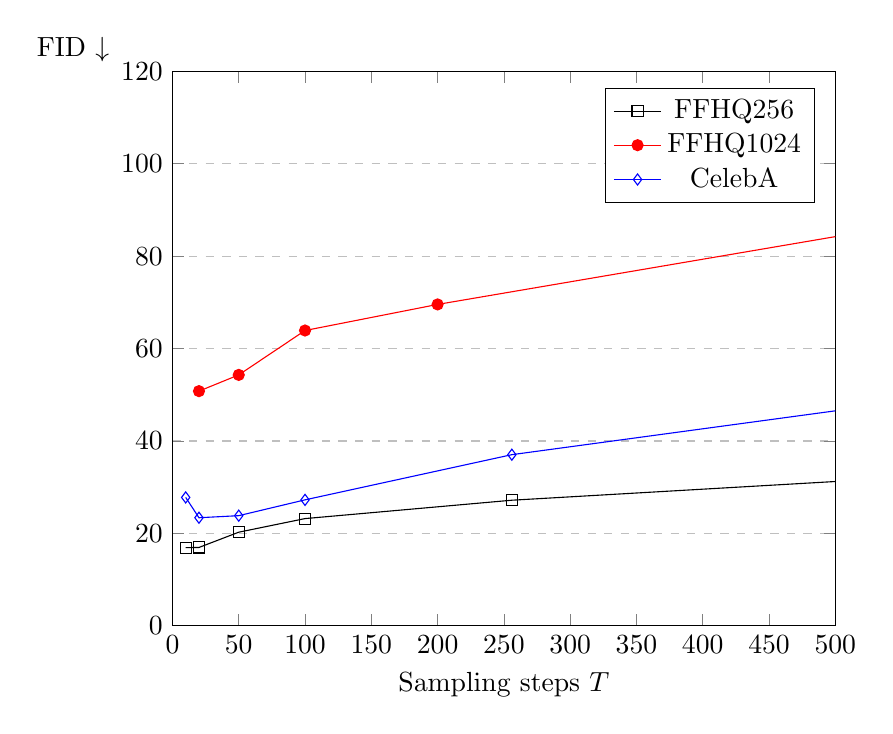
\begin{tikzpicture}
\begin{axis}[
y label style={at={(axis description cs:-0.15,1.0)},rotate=-90,anchor=south},
title={},
xlabel={Sampling steps $T$},
ylabel={FID $\downarrow$},
xmin=0, xmax=500,
ymin=0, ymax=120,
xtick={0,50,100,150,200,250,300,350,400,450,500},
ytick={0,20,40,60,80,100,120},
legend pos=north east,
ymajorgrids=true,
grid style=dashed,
]\addplot[color=black, mark=square]
coordinates {(10.0, 16.933240853331633)(20.0, 16.968015496794585)(50.0, 20.269439432847413)(100.0, 23.214299375538577)(256.0, 27.189009006094718)(512.0, 31.435942790814245)};
\addlegendentry{FFHQ256}
\addplot[color=red, mark=*]
coordinates {(20.0, 50.79169256114352)(50.0, 54.30311107720983)(100.0, 63.90726480083863)(200.0, 69.5533429056805)(512.0, 84.80617604620527)(1024.0, 100.93734948403663)};
\addlegendentry{FFHQ1024}
\addplot[color=blue, mark=diamond]
coordinates {(10.0, 27.79389706651663)(20.0, 23.397719254573232)(50.0, 23.845846223411986)(100.0, 27.26720576724899)(256.0, 37.0436486740923)(512.0, 46.99500404006332)};
\addlegendentry{CelebA}
\end{axis}
\end{tikzpicture}

        }
        \caption{Steps vs. FID}
    \end{subfigure}
    \hfill
    \begin{subfigure}[b]{0.33\textwidth}
        \centering
        \resizebox{\textwidth}{!}{
            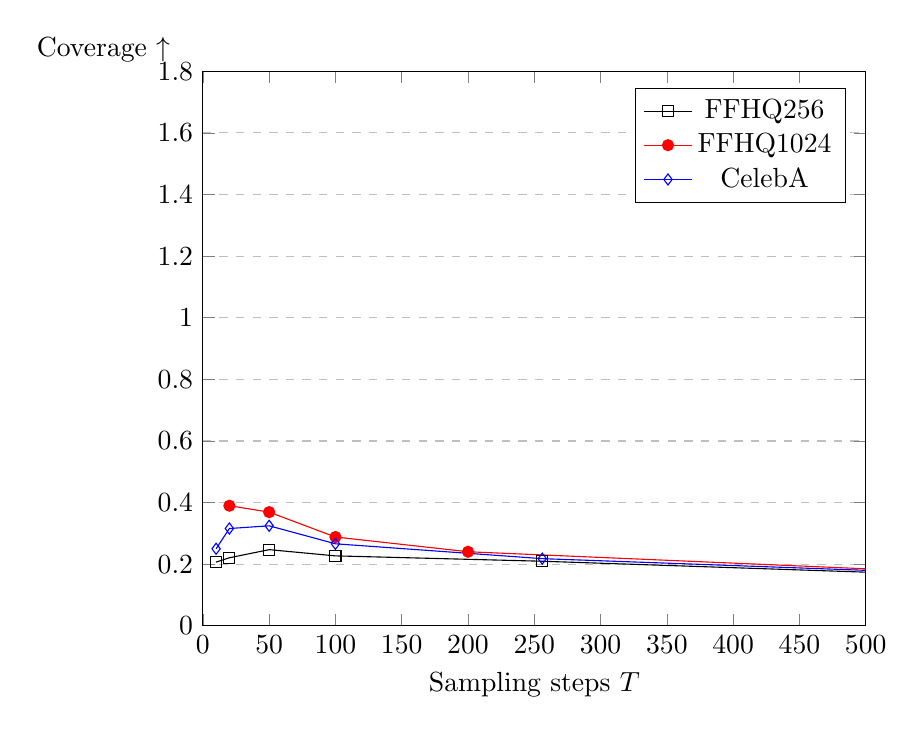
\begin{tikzpicture}
\begin{axis}[
y label style={at={(axis description cs:-0.15,1.0)},rotate=-90,anchor=south},
title={},
xlabel={Sampling steps $T$},
ylabel={Coverage $\uparrow$},
xmin=0, xmax=500,
ymin=0.0, ymax=1.8,
xtick={0,50,100,150,200,250,300,350,400,450,500},
ytick={0.0,0.2,0.4,0.6000000000000001,0.8,1.0,1.2000000000000002,1.4000000000000001,1.6,1.8},
legend pos=north east,
ymajorgrids=true,
grid style=dashed,
]\addplot[color=black, mark=square]
coordinates {(10.0, 0.207)(20.0, 0.221)(50.0, 0.2474)(100.0, 0.2272)(256.0, 0.2098)(512.0, 0.1726)};
\addlegendentry{FFHQ256}
\addplot[color=red, mark=*]
coordinates {(20.0, 0.39)(50.0, 0.3692)(100.0, 0.2884)(200.0, 0.2406)(512.0, 0.183)(1024.0, 0.1448)};
\addlegendentry{FFHQ1024}
\addplot[color=blue, mark=diamond]
coordinates {(10.0, 0.2502)(20.0, 0.316)(50.0, 0.3248)(100.0, 0.2664)(256.0, 0.2182)(512.0, 0.1784)};
\addlegendentry{CelebA}
\end{axis}
\end{tikzpicture}

        }
        \caption{Steps vs. Coverage}
    \end{subfigure}
    \hfill
    \begin{subfigure}[b]{0.33\textwidth}
        \centering
        \resizebox{\textwidth}{!}{
            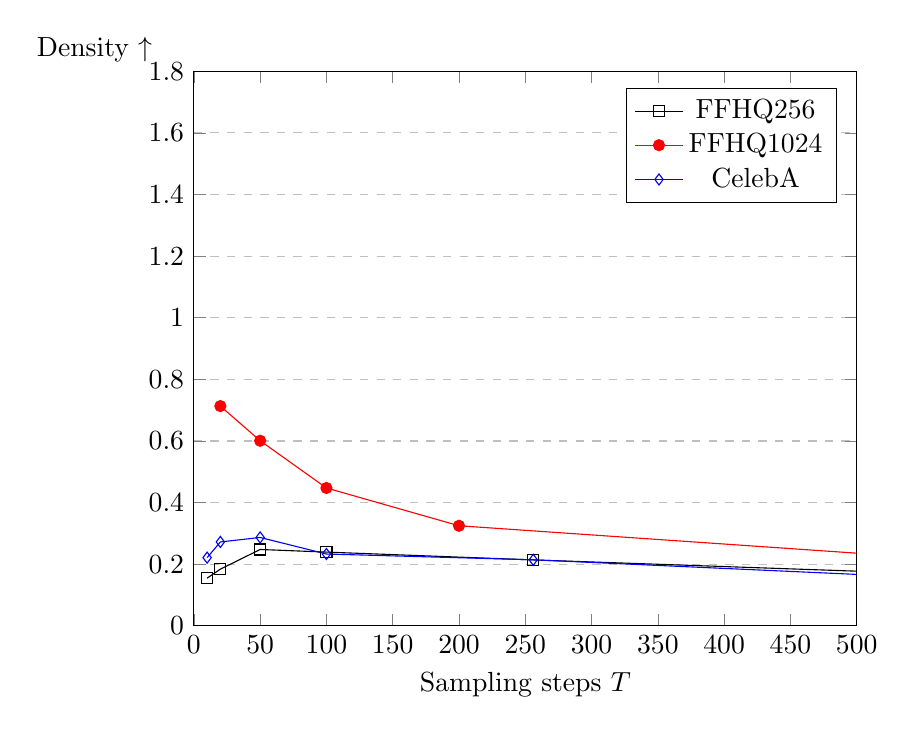
\begin{tikzpicture}
\begin{axis}[
y label style={at={(axis description cs:-0.15,1.0)},rotate=-90,anchor=south},
title={},
xlabel={Sampling steps $T$},
ylabel={Density $\uparrow$},
xmin=0, xmax=500,
ymin=0.0, ymax=1.8,
xtick={0,50,100,150,200,250,300,350,400,450,500},
ytick={0.0,0.2,0.4,0.6000000000000001,0.8,1.0,1.2000000000000002,1.4000000000000001,1.6,1.8},
legend pos=north east,
ymajorgrids=true,
grid style=dashed,
]\addplot[color=black, mark=square]
coordinates {(10.0, 0.155)(20.0, 0.18413333333333332)(50.0, 0.24793333333333334)(100.0, 0.23946666666666666)(256.0, 0.21406666666666666)(512.0, 0.17573333333333332)};
\addlegendentry{FFHQ256}
\addplot[color=red, mark=*]
coordinates {(20.0, 0.7133333333333334)(50.0, 0.6008666666666667)(100.0, 0.44753333333333334)(200.0, 0.3249333333333333)(512.0, 0.2324)(1024.0, 0.16773333333333332)};
\addlegendentry{FFHQ1024}
\addplot[color=blue, mark=diamond]
coordinates {(10.0, 0.2215333333333333)(20.0, 0.2724)(50.0, 0.2869333333333333)(100.0, 0.2332)(256.0, 0.21446666666666664)(512.0, 0.16473333333333331)};
\addlegendentry{CelebA}
\end{axis}
\end{tikzpicture}

        }
        \caption{Steps vs. Density}
    \end{subfigure}
    \caption{
        Plots showing sample quality in terms of different metrics as
        number of sampling steps $\markovSteps$ increases. Counter-intuitively, the
        sample quality decreases with number of sampling steps, seen on
        all metrics and datasets.
    }
\end{figure}

\begin{figure}[ht!]
    \begin{subfigure}[b]{0.33\textwidth}
        \centering
        \resizebox{\textwidth}{!}{
            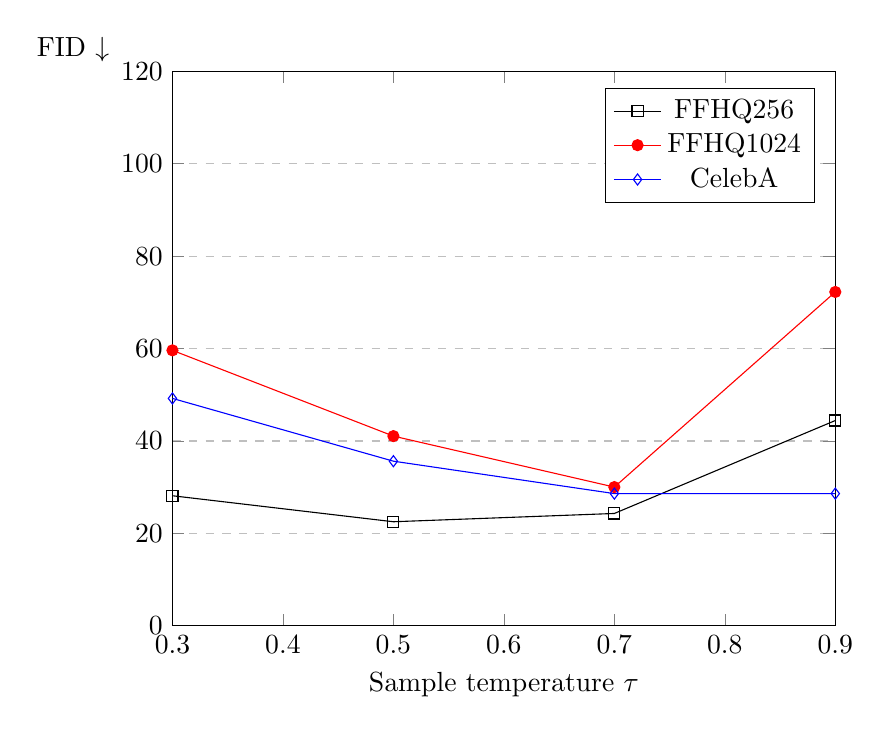
\begin{tikzpicture}
\begin{axis}[
y label style={at={(axis description cs:-0.15,1.0)},rotate=-90,anchor=south},
title={},
xlabel={Sample temperature $\tau$},
ylabel={FID $\downarrow$},
xmin=0.3, xmax=0.9000000000000001,
ymin=0, ymax=120,
xtick={0.3,0.4,0.5,0.6000000000000001,0.7000000000000002,0.8000000000000003,0.9000000000000001},
ytick={0,20,40,60,80,100,120},
legend pos=north east,
ymajorgrids=true,
grid style=dashed,
]\addplot[color=black, mark=square]
coordinates {(1.0, 83.59790014438649)(0.9, 44.43439367176743)(0.7, 24.322136621661407)(0.5, 22.530204016446124)(0.3, 28.155348332963445)};
\addlegendentry{FFHQ256}
\addplot[color=red, mark=*]
coordinates {(1.0, 281.35575866892975)(0.9, 72.24972119845785)(0.7, 30.030630965588852)(0.5, 41.06155796980428)(0.3, 59.61624309496067)};
\addlegendentry{FFHQ1024}
\addplot[color=blue, mark=diamond]
coordinates {(1.0, 75.80203954506536)(0.9, 28.617311837121477)(0.7, 28.621503391331398)(0.5, 35.63571015802388)(0.3, 49.21726306807049)};
\addlegendentry{CelebA}
\end{axis}
\end{tikzpicture}

        }
        \caption{Temperature $\temperature$ vs. FID}
    \end{subfigure}
    \hfill
    \begin{subfigure}[b]{0.33\textwidth}
        \centering
        \resizebox{\textwidth}{!}{
            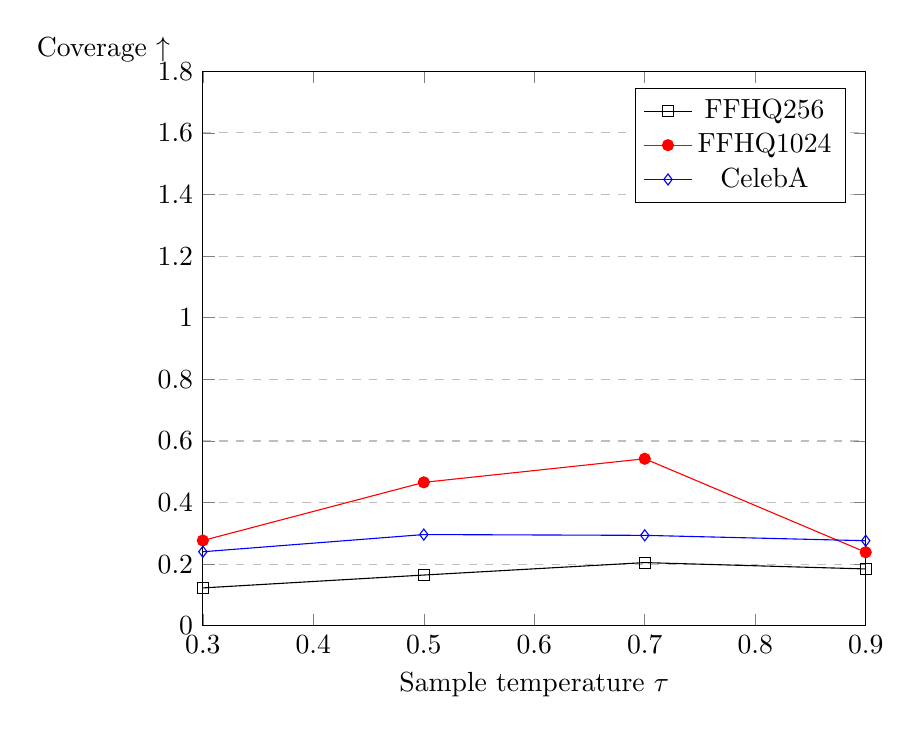
\begin{tikzpicture}
\begin{axis}[
y label style={at={(axis description cs:-0.15,1.0)},rotate=-90,anchor=south},
title={},
xlabel={Sample temperature $\tau$},
ylabel={Coverage $\uparrow$},
xmin=0.3, xmax=0.9000000000000001,
ymin=0.0, ymax=1.8,
xtick={0.3,0.4,0.5,0.6000000000000001,0.7000000000000002,0.8000000000000003,0.9000000000000001},
ytick={0.0,0.2,0.4,0.6000000000000001,0.8,1.0,1.2000000000000002,1.4000000000000001,1.6,1.8},
legend pos=north east,
ymajorgrids=true,
grid style=dashed,
]\addplot[color=black, mark=square]
coordinates {(1.0, 0.0662)(0.9, 0.1848)(0.7, 0.2054)(0.5, 0.165)(0.3, 0.1232)};
\addlegendentry{FFHQ256}
\addplot[color=red, mark=*]
coordinates {(1.0, 0.0004)(0.9, 0.239)(0.7, 0.5424)(0.5, 0.4658)(0.3, 0.277)};
\addlegendentry{FFHQ1024}
\addplot[color=blue, mark=diamond]
coordinates {(1.0, 0.124)(0.9, 0.2764)(0.7, 0.2938)(0.5, 0.2964)(0.3, 0.2406)};
\addlegendentry{CelebA}
\end{axis}
\end{tikzpicture}

        }
        \caption{Temperature $\temperature$ vs. Coverage}
    \end{subfigure}
    \hfill
    \begin{subfigure}[b]{0.33\textwidth}
        \centering
        \resizebox{\textwidth}{!}{
            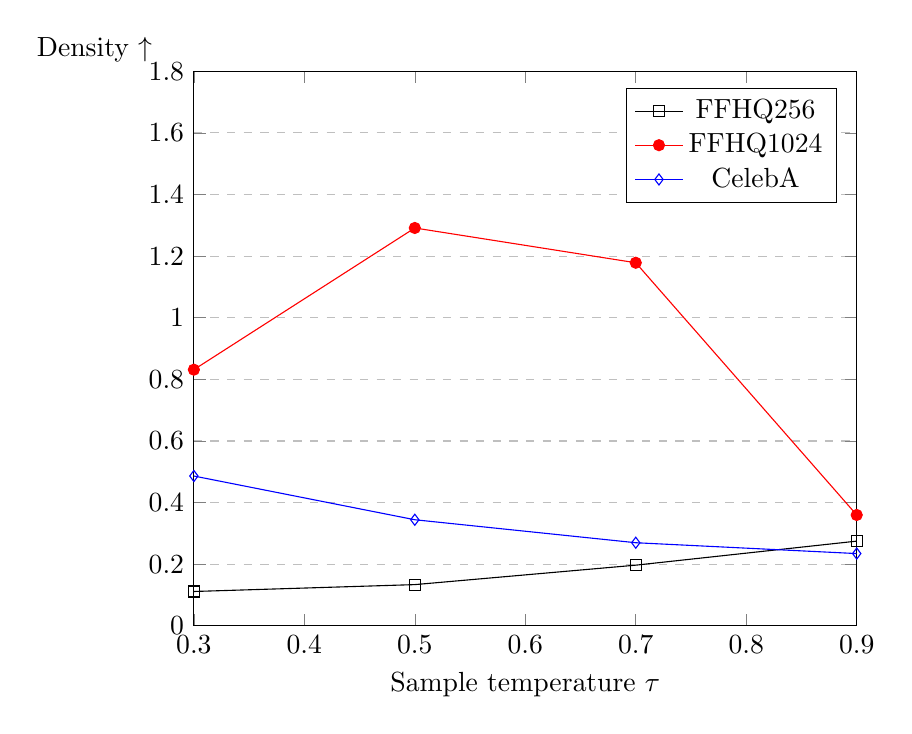
\begin{tikzpicture}
\begin{axis}[
y label style={at={(axis description cs:-0.15,1.0)},rotate=-90,anchor=south},
title={},
xlabel={Sample temperature $\tau$},
ylabel={Density $\uparrow$},
xmin=0.3, xmax=0.9000000000000001,
ymin=0.0, ymax=1.8,
xtick={0.3,0.4,0.5,0.6000000000000001,0.7000000000000002,0.8000000000000003,0.9000000000000001},
ytick={0.0,0.2,0.4,0.6000000000000001,0.8,1.0,1.2000000000000002,1.4000000000000001,1.6,1.8},
legend pos=north east,
ymajorgrids=true,
grid style=dashed,
]\addplot[color=black, mark=square]
coordinates {(1.0, 0.07566666666666666)(0.9, 0.2750666666666667)(0.7, 0.19706666666666664)(0.5, 0.13393333333333332)(0.3, 0.11159999999999999)};
\addlegendentry{FFHQ256}
\addplot[color=red, mark=*]
coordinates {(1.0, 0.00019999999999999998)(0.9, 0.3599333333333333)(0.7, 1.1785333333333332)(0.5, 1.2913999999999999)(0.3, 0.8315333333333333)};
\addlegendentry{FFHQ1024}
\addplot[color=blue, mark=diamond]
coordinates {(1.0, 0.12519999999999998)(0.9, 0.23466666666666663)(0.7, 0.26986666666666664)(0.5, 0.3444666666666667)(0.3, 0.4864)};
\addlegendentry{CelebA}
\end{axis}
\end{tikzpicture}

        }
        \caption{Temperature $\temperature$ vs. Density}
    \end{subfigure}
    \caption{
        Plots showing sample quality in terms of different metrics as sample
        temperature $\temperature$ is changed. Given the other parameters, a good choice
        of $\temperature$ falls in the range $0.5-0.7$. However, this range may
        differ depending on the other choice of parameters.
    }
\end{figure}

\begin{figure}[ht!]
    \begin{subfigure}[b]{0.33\textwidth}
        \centering
        \resizebox{\textwidth}{!}{
            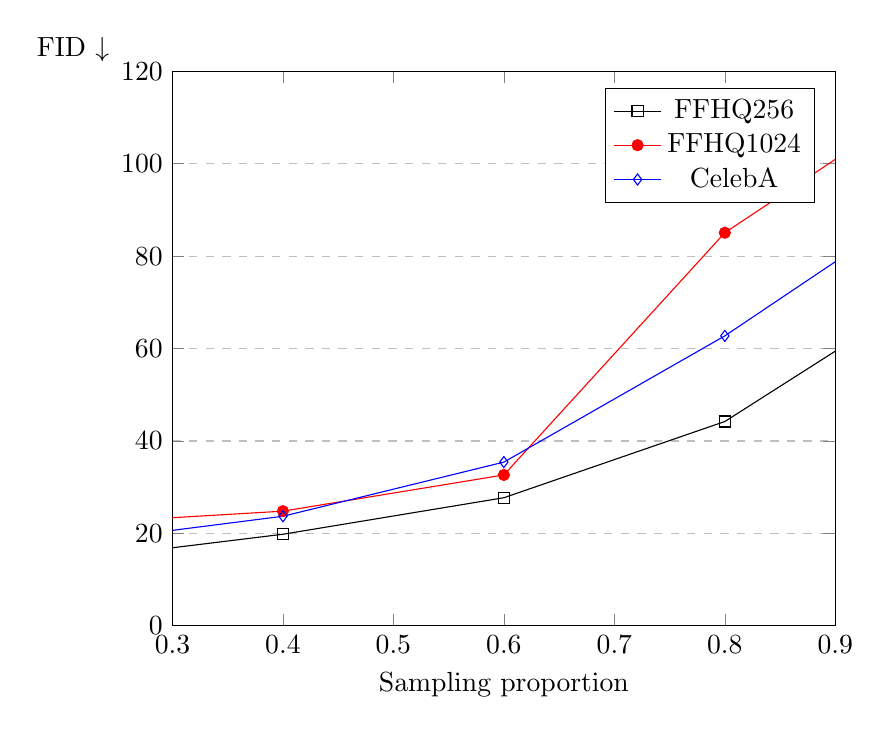
\begin{tikzpicture}
\begin{axis}[
y label style={at={(axis description cs:-0.15,1.0)},rotate=-90,anchor=south},
title={},
xlabel={Sampling proportion},
ylabel={FID $\downarrow$},
xmin=0.3, xmax=0.9000000000000001,
ymin=0, ymax=120,
xtick={0.3,0.4,0.5,0.6000000000000001,0.7000000000000002,0.8000000000000003,0.9000000000000001},
ytick={0,20,40,60,80,100,120},
legend pos=north east,
ymajorgrids=true,
grid style=dashed,
]\addplot[color=black, mark=square]
coordinates {(1.0, 74.66283778948849)(0.8, 44.21927055440783)(0.6, 27.725188336835213)(0.4, 19.825740890874904)(0.2, 13.976620506685805)};
\addlegendentry{FFHQ256}
\addplot[color=red, mark=*]
coordinates {(1.0, 116.81614755529716)(0.8, 85.06652266724691)(0.6, 32.65933412137353)(0.4, 24.82419203797879)(0.2, 21.979835694569083)};
\addlegendentry{FFHQ1024}
\addplot[color=blue, mark=diamond]
coordinates {(1.0, 94.83723271911529)(0.8, 62.7489179950907)(0.6, 35.43514345702618)(0.4, 23.718088259439654)(0.2, 17.614758693266793)};
\addlegendentry{CelebA}
\end{axis}
\end{tikzpicture}

        }
        \caption{Sample proportion vs. FID}
    \end{subfigure}
    \hfill
    \begin{subfigure}[b]{0.33\textwidth}
        \centering
        \resizebox{\textwidth}{!}{
            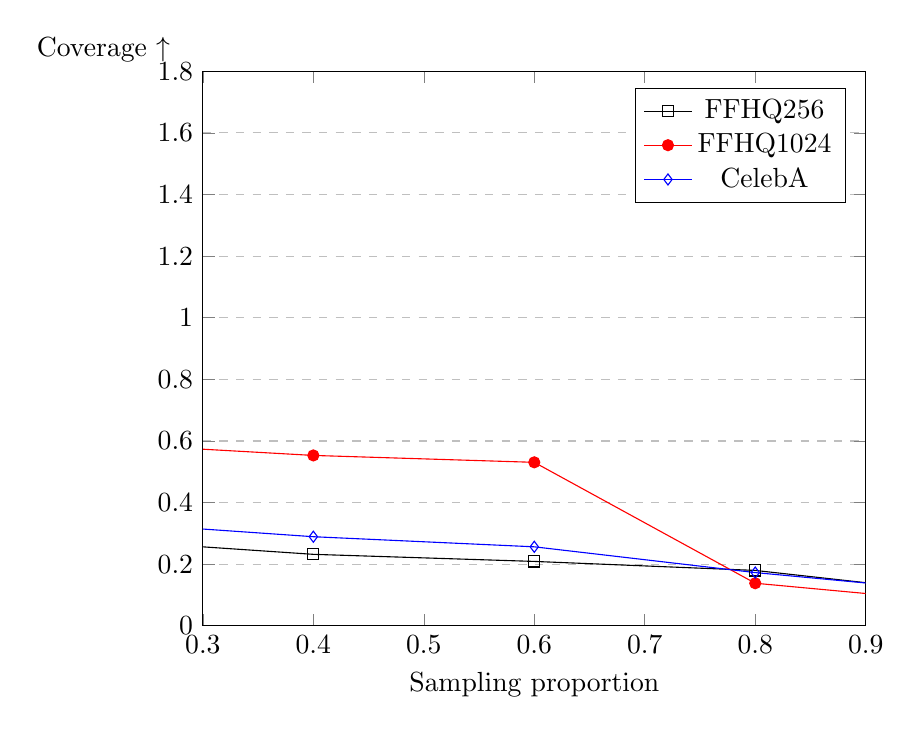
\begin{tikzpicture}
\begin{axis}[
y label style={at={(axis description cs:-0.15,1.0)},rotate=-90,anchor=south},
title={},
xlabel={Sampling proportion},
ylabel={Coverage $\uparrow$},
xmin=0.3, xmax=0.9000000000000001,
ymin=0.0, ymax=1.8,
xtick={0.3,0.4,0.5,0.6000000000000001,0.7000000000000002,0.8000000000000003,0.9000000000000001},
ytick={0.0,0.2,0.4,0.6000000000000001,0.8,1.0,1.2000000000000002,1.4000000000000001,1.6,1.8},
legend pos=north east,
ymajorgrids=true,
grid style=dashed,
]\addplot[color=black, mark=square]
coordinates {(1.0, 0.1002)(0.8, 0.18)(0.6, 0.2092)(0.4, 0.2322)(0.2, 0.2808)};
\addlegendentry{FFHQ256}
\addplot[color=red, mark=*]
coordinates {(1.0, 0.0718)(0.8, 0.1384)(0.6, 0.5308)(0.4, 0.5532)(0.2, 0.5936)};
\addlegendentry{FFHQ1024}
\addplot[color=blue, mark=diamond]
coordinates {(1.0, 0.1054)(0.8, 0.173)(0.6, 0.2566)(0.4, 0.2894)(0.2, 0.3392)};
\addlegendentry{CelebA}
\end{axis}
\end{tikzpicture}

        }
        \caption{Sample proportion vs. Coverage}
    \end{subfigure}
    \hfill
    \begin{subfigure}[b]{0.33\textwidth}
        \centering
        \resizebox{\textwidth}{!}{
            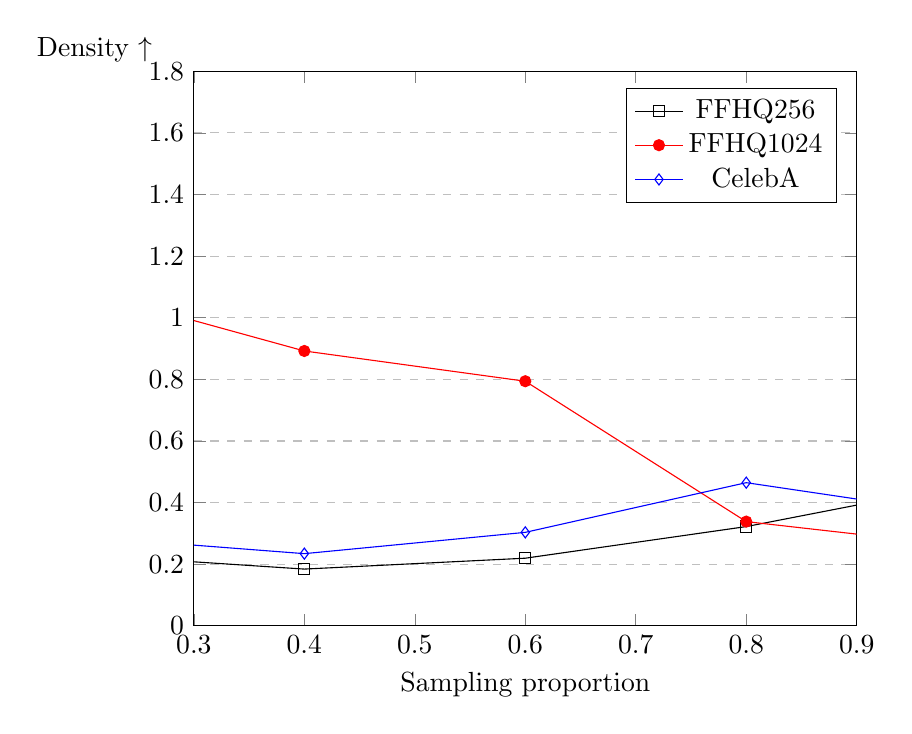
\begin{tikzpicture}
\begin{axis}[
y label style={at={(axis description cs:-0.15,1.0)},rotate=-90,anchor=south},
title={},
xlabel={Sampling proportion},
ylabel={Density $\uparrow$},
xmin=0.3, xmax=0.9000000000000001,
ymin=0.0, ymax=1.8,
xtick={0.3,0.4,0.5,0.6000000000000001,0.7000000000000002,0.8000000000000003,0.9000000000000001},
ytick={0.0,0.2,0.4,0.6000000000000001,0.8,1.0,1.2000000000000002,1.4000000000000001,1.6,1.8},
legend pos=north east,
ymajorgrids=true,
grid style=dashed,
]\addplot[color=black, mark=square]
coordinates {(1.0, 0.46173333333333333)(0.8, 0.32226666666666665)(0.6, 0.21966666666666668)(0.4, 0.18433333333333335)(0.2, 0.23146666666666665)};
\addlegendentry{FFHQ256}
\addplot[color=red, mark=*]
coordinates {(1.0, 0.25726666666666664)(0.8, 0.33840000000000003)(0.6, 0.794)(0.4, 0.8922)(0.2, 1.0897333333333332)};
\addlegendentry{FFHQ1024}
\addplot[color=blue, mark=diamond]
coordinates {(1.0, 0.35853333333333326)(0.8, 0.4648)(0.6, 0.3035333333333333)(0.4, 0.2344)(0.2, 0.2897333333333333)};
\addlegendentry{CelebA}
\end{axis}
\end{tikzpicture}

        }
        \caption{Sample proportion vs. Density}
    \end{subfigure}
    \caption{
        Plots showing sample quality in terms of different metrics as sample
        proportion is changed. Lower values seem to perform better given the
        other parameters, but again the optimal range may differ if other
        parameters are changed.
    }
\end{figure}

\begin{figure}[ht]
    \centering
    \begin{subfigure}[b]{0.47\textwidth}
        \centering
        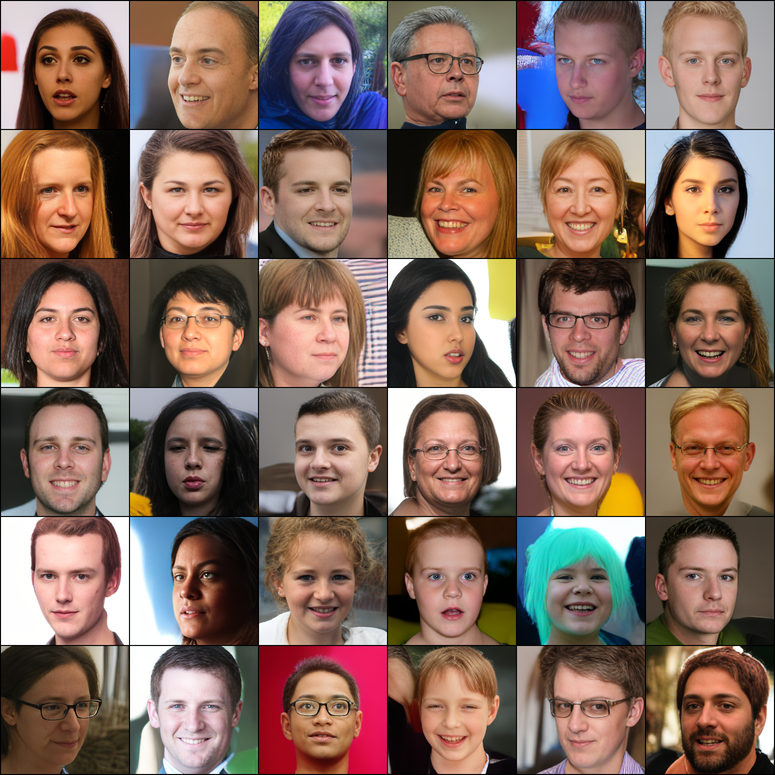
\includegraphics[width=1.0\textwidth]{figures/ffhq256-samples-small.png}
        \caption{
            Non-cherry picked batch of samples from the model trained on FFHQ256.
        }
    \end{subfigure}
    \hfill
    \begin{subfigure}[b]{0.47\textwidth}
        \centering
        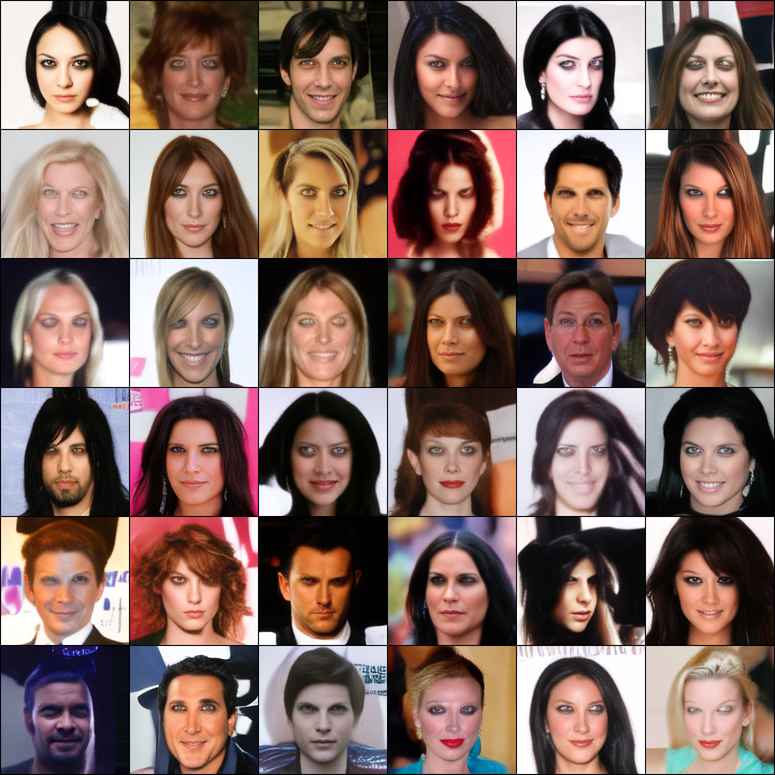
\includegraphics[width=1.0\textwidth]{figures/celeba-samples-small.png}
        \caption{
            Non-cherry picked batch of samples from the model trained on CelebA.
        }
    \end{subfigure}
    \caption{Unconditional generation on $256 \times 256$ face datasets.}
\end{figure}

\begin{figure}[ht]
    \centering
    \begin{subfigure}[b]{\textwidth}
        \centering
        \includegraphics[width=1.0\textwidth]{figures/nearest-ffhq256.png}
        \caption{
            FFHQ256 samples and nearest neighbours from the dataset, based on LPIPS
            perceptual loss. Left-most column is a sample from our trained
            model, followed then by nearest neighbours, increasing in distance
            from left-to-right.
        }
    \end{subfigure}
\end{figure}

\subsection{Conditional Image Generation}

\begin{figure}[ht]
    \centering
    \begin{subfigure}[b]{0.47\textwidth}
        \centering
        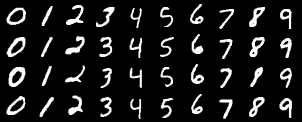
\includegraphics[width=1.0\textwidth]{figures/mnist-samples.png}
        \caption{
            Conditional, pixel-wise generation on MNIST.
        }
    \end{subfigure}
    \hfill
    \begin{subfigure}[b]{0.47\textwidth}
        \centering
        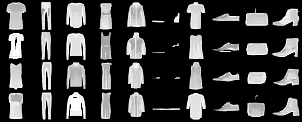
\includegraphics[width=1.0\textwidth]{figures/fashionmnist-samples.png}
        \caption{
            Conditional, pixel-wise generation on Fashion-MNIST.
        }
    \end{subfigure}
    \caption{
        Testing conditional generation using MNIST-style datasets. Coherent
        samples demonstrate that the proposed conditioning method does inject class
        information.
    }
    \label{fig:mnist}
\end{figure}

Another critical component of an ideal generative model is the ability to
control its generation. We explore class-conditioned image generation of
ImageNet at $256 \times 256$ resolution, using the pretrained ImageNet
\gls{vqgan} checkpoints provided by the original work~\cite{esser2021taming}. 

There are many ways to integrate class conditioning to a generative model. One
solution is to pass a one-hot or embedding vector of the classes as an auxiliary
input to the model. We use another simple solution, to add an additional
embedding layer containing one embedding for each of the 1000 classes present in
ImageNet. This approach was done in Image Transformer~\cite{parmar2018image} and
was found to be effective. 

It was not immediately apparent whether this method would also work for
\gls{sundae}, so before running expensive ImageNet experiments we first did some
preliminary experiments on class-conditioned, pixel-wise, \gls{nar} generation
on two MNIST-style datasets: MNIST and Fashion-MNIST. These experiments can be
done, despite not having an associated \gls{vqgan} model, by treating each
possible 8-bit greyscale colour as if it were an index into a discrete codebook
of size $2^8$. Once sampled, we simply output the discrete values directly to
produce a final image. These preliminary experiments showed us that \gls{sundae}
can successfully use class information using this simple approach, seen in
Figure~\ref{fig:mnist}.

\begin{figure}[ht]
    \centering
    \begin{subfigure}[b]{0.47\textwidth}
        \centering
        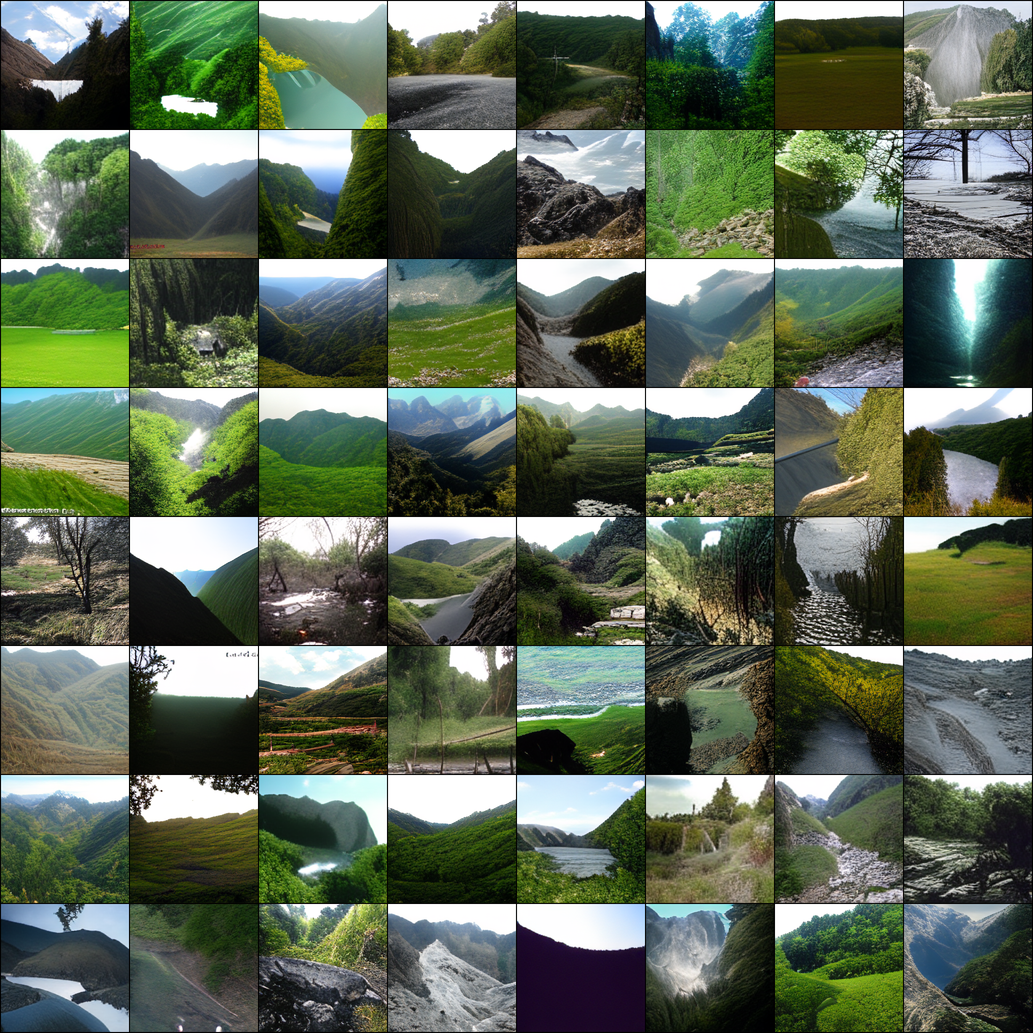
\includegraphics[width=1.0\textwidth]{figures/imagenet-valley-small.png}
        \caption{
            $256 \times 256$ successful samples from the class ``Valley''.}
    \end{subfigure}
    \hfill
    \begin{subfigure}[b]{0.47\textwidth}
        \centering
        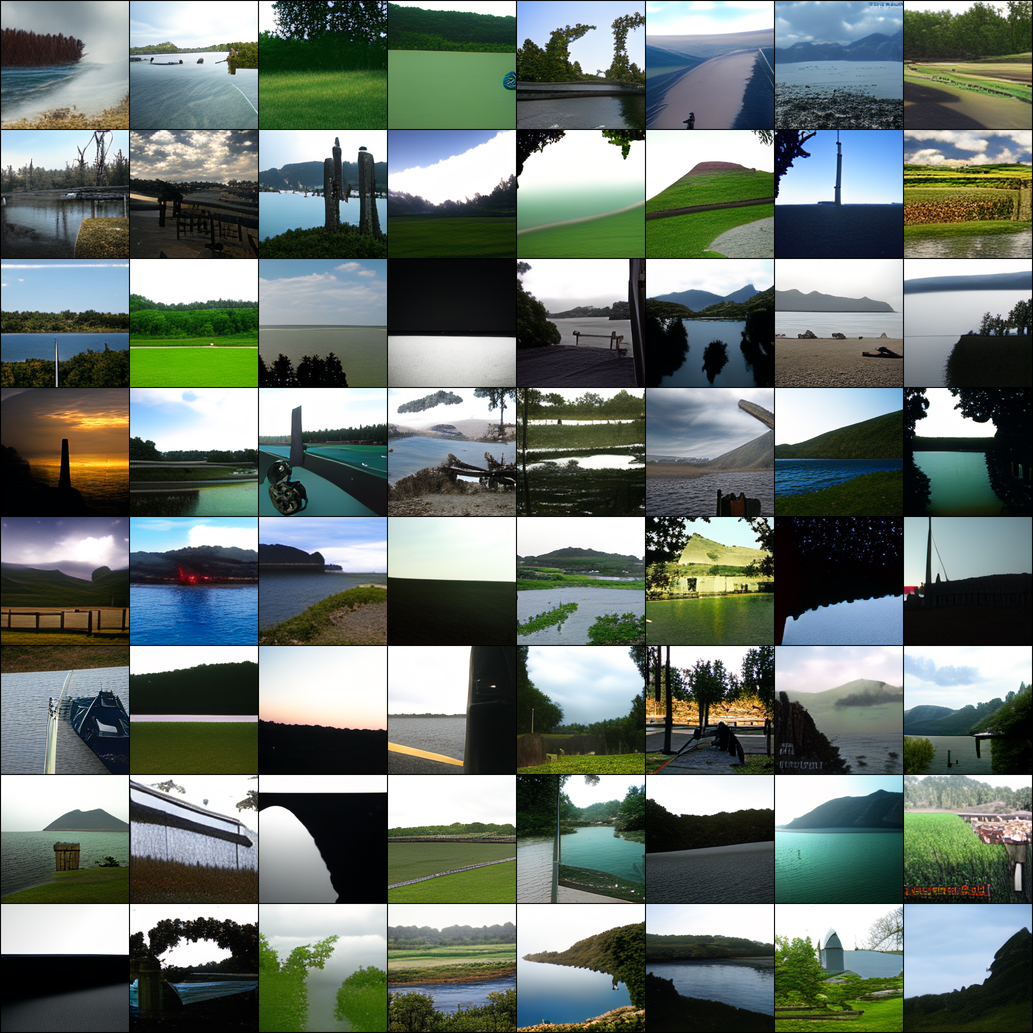
\includegraphics[width=1.0\textwidth]{figures/imagenet-lakeside-small.png}
        \caption{
            $256 \times 256$ successful samples from the class ``Lakeside''.
        }
    \end{subfigure}\\
    \vspace{0.5cm}
    \begin{subfigure}[b]{0.47\textwidth}
        \centering
        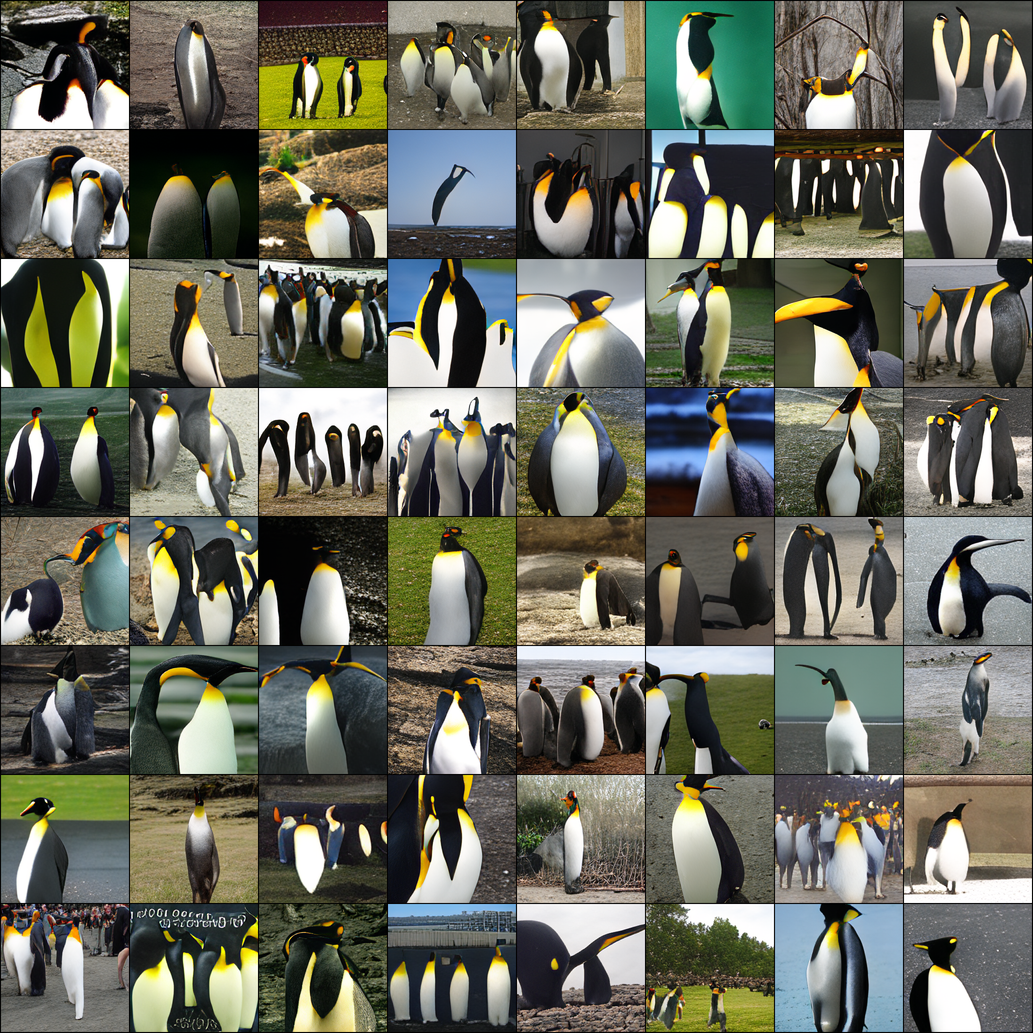
\includegraphics[width=1.0\textwidth]{figures/imagenet-penguin-small.png}
        \caption{
            $256 \times 256$ failed samples from the class ``King Penguin''.
        }
    \end{subfigure}
    \hfill
    \begin{subfigure}[b]{0.47\textwidth}
        \centering
        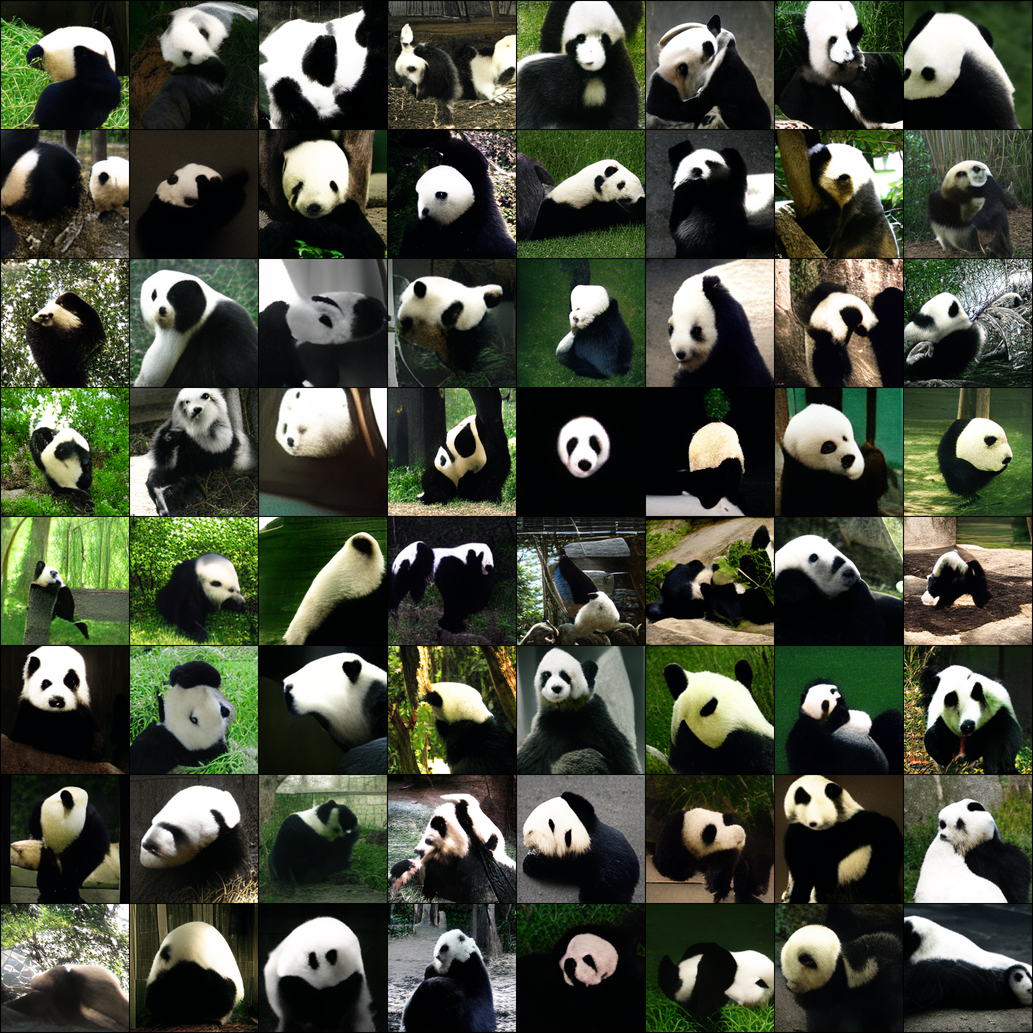
\includegraphics[width=1.0\textwidth]{figures/imagenet-panda-small.png}
        \caption{
            $256 \times 256$ failed samples from the class ``Giant Panda''.
        }
    \end{subfigure}
    \caption{Examples of class-conditioned generation on ImageNet using
        $\markovSteps = 50$ sampling steps. Top row contains examples of
    successful samples whereas bottom row showed failed samples. The contents of
    the failed samples nonetheless do resemble the target class.}
    \label{fig:imagenet}
\end{figure}

A relatively new method of providing a conditioning signal is to instead provide
natural language prompts, and learn the joint distribution of prompts and
images. At inference time, this allows for text-to-image generation which in
turn allows for zero-shot image generation given a sufficiently sized training
dataset. Most notably, DALL·E~\cite{ramesh2021dalle} and recently
DALL·E-2~\cite{ramesh2022dalle2}, with the former generating VQ-VAE discrete
latents and the latter generating continuous \textit{``CLIP Image embeddings''}.
DALL·E-2 was able to produce high fidelity samples at $1024 \times 1024$
resolution. Concurrently, Latent Diffusion
Models~\cite{rombach2021highresolution} used text embeddings to condition
sampling, again allowing for zero-shot generation. Our model is also capable of
using such methods, turning our model from an unconditional or class-conditioned
generative model to a text-to-image generative model. However, due to
time-constraints we did not experiment with this approach, leaving this for
future work.

\subsection{Arbitrary Image Inpainting}

As outlined earlier, \acrlong{nar} generative models have a number of advantages
on inpainting tasks, including supporting arbitrary masks and being able to use
the full context available to them. We provide a number of examples of
inpainting on FFHQ1024 and ImageNet, showcasing different patterns and different
results given the same starting image. As our method utilises a vector quantized
image model, it is incapable of doing fine-grained inpainting at a pixel level.
Nonetheless, the results show consistently good inpainting results when
operating at a \gls{vq} latent level.

\begin{figure}[ht]
    \centering
    \begin{subfigure}[b]{\textwidth}
        \centering
        \label{fig:inpaintExample}
        \includegraphics[width=1.0\linewidth]{figures/inpaint.png}
        \caption{A large example of inpainting on a $1024 \times 1024$ image using our
        model.}
    \end{subfigure}
    \\
    \begin{subfigure}[b]{0.47\textwidth}
        \centering
        \includegraphics[width=1.0\textwidth]{figures/inpaint-block/inpaint-variation-small.png}
        \caption{
            Multiple outputs of inpainting using the same block mask.
        }
    \end{subfigure}
    \hfill
    \begin{subfigure}[b]{0.47\textwidth}
        \centering
        \includegraphics[width=1.0\textwidth]{figures/inpaint-rand/inpaint-variation-small.png}
        \caption{
            Multiple outputs of inpainting on the same random mask. 
        }
    \end{subfigure}
    \caption{
        Inpainting results on FFHQ-1024. We compute multiple outputs per
        input image and mask to demonstrate diversity of outputs. Inpainting
        using a \gls{vq} image model cannot be applied perfectly at a
        pixel-level. Nevertheless, the model still produces many convincing
        outputs at very high resolutions.
    }
\end{figure}



\section{Conclusion}\label{sec:conclusion}
In this work we investigated pushing the efficiency of generative models via the
combination of various techniques, following the general trend in generative
modelling of simultaneously improving quality and speed of sampling using
non-adversarial approaches. We found that the combination of these techniques
formed a fast image generation framework. To our surprise, the proposed method
was faster and more scaleable than expected, able to be applied with ease to
megapixel images, and generate samples at such resolutions in seconds -- a wide
margin faster than prior non-adversarial methods. Additionally, we found that
previously proposed hourglass transformers are not optimally defined on
multi-dimensional inputs and subsequently proposed adjustments to them. Our work
demonstrates the superiority of the \acrlong{nar} paradigm, and joins a rapidly
growing space of research into their use as a viable alternative to \acrlong{ar}
frameworks. Additional research is needed into better \gls{vq} image models and
into a stronger conditional generative model.


\bibliographystyle{iclr2022_conference}
{\small \bibliography{references}}

\end{document}
